\documentclass[11pt, a4paper, twocolumn]{article}

\usepackage[top=2cm, bottom=2cm, left=1.5cm, right=1.5cm, columnsep=0.6cm]{geometry}
\usepackage{graphicx}
\usepackage{booktabs}
\usepackage{amsmath}
\usepackage{hyperref}
\usepackage{caption}
\usepackage{subcaption}
\usepackage{natbib}
\usepackage{parskip}
\usepackage{titlesec}
\usepackage{array}
\usepackage{microtype}
\usepackage{xcolor}
\usepackage{abstract}
\usepackage{fancyhdr}
\usepackage{times}

\hypersetup{colorlinks=true, linkcolor=black, citecolor=blue, urlcolor=blue}

\captionsetup{font=footnotesize, labelfont=bf, justification=justified}
\graphicspath{{figures/}}

\titleformat{\section}{\normalsize\bfseries\scshape}{\thesection.}{0.4em}{}
\titleformat{\subsection}{\normalsize\bfseries}{\thesubsection.}{0.4em}{}
\titleformat{\subsubsection}{\small\itshape}{\thesubsubsection.}{0.4em}{}
\titlespacing{\section}{0pt}{6pt}{3pt}
\titlespacing{\subsection}{0pt}{4pt}{2pt}
\titlespacing{\subsubsection}{0pt}{3pt}{1pt}

\setlength{\parskip}{3pt}
\setlength{\parindent}{0pt}

\renewcommand{\abstractnamefont}{\normalfont\bfseries\scshape}
\renewcommand{\abstracttextfont}{\small}
\setlength{\absleftindent}{0pt}
\setlength{\absrightindent}{0pt}

\pagestyle{fancy}
\fancyhf{}
\renewcommand{\headrulewidth}{0.4pt}
\fancyhead[L]{\footnotesize Human Brain Mapping -- Assignment 3}
\fancyhead[R]{\footnotesize P300 ERP Analysis}
\fancyfoot[C]{\thepage}

\title{\textbf{Electrophysiological Dynamics and ERP Analysis: P300 in an Auditory Oddball Paradigm}\\[0.3em]
{\small \textit{Human Brain Mapping: Assignment 3 }}}
\author{Arya Shah (25290002)}
\date{}

\begin{document}

  \maketitle
  \begin{abstract}
    \noindent This report describes the preprocessing, ERP analysis, and reference-scheme comparison of a single-subject 64-channel EEG dataset recorded during an auditory three-stimulus oddball paradigm. After bandpass filtering (1--40~Hz), notch filtering (50~Hz), bad channel interpolation (T7), and ICA-based artifact removal (5 components), 741 of 747 trials were retained. The oddball condition elicited a robust P300 component peaking at 406.2~ms at Pz with a mean amplitude of $+4.66\ \mu$V in the 300--500~ms window, significantly larger than both the noise ($d = 1.14$) and standard ($d = 1.46$) conditions, $F(2, 738) = 103.86$, $p < .001$. A topographic comparison across five reference schemes confirms that average referencing provides the most accurate representation of the P300 scalp distribution and is optimal for occipito-temporal sensor mapping.
    \vspace{0.5em}
  \end{abstract}
  \vspace{-0.5em}
  \vspace{0.5em}

\section{Introduction and Research Question}

The P300 (or P3) is one of the most studied event-related potential (ERP)
components in cognitive neuroscience. It appears as a positive deflection
over centro-parietal scalp electrodes roughly 300 to 600 milliseconds
after a task-relevant stimulus. It was first described by \citet{Sutton1965}
and has since been interpreted as a neural marker of attentional resource
allocation, context updating in working memory, and conscious target
detection \citep{Donchin1988, Polich2007}.

The dataset used here comes from a single participant (sub-001) recorded at
the Meditation Research Institute, Rishikesh, India. The task was a
classic three-stimulus auditory oddball paradigm. Participants heard three
types of sounds: frequent standards (500~Hz pure tone, 70\%), rare oddballs
(1000~Hz pure tone, 15\%), and distractors (white noise, 15\%). They were
instructed to press a button whenever they heard the oddball and to ignore
all other sounds. Data were recorded with a Biosemi Active Two system at
256~Hz using a 64-channel biosemi64 cap.

\textbf{Research Question:} Does the P300 component at centro-parietal
electrodes differ in mean amplitude across the three stimulus conditions
(standard, oddball, noise) in the 300--500~ms time window, and if so,
does this reflect target-specific neural processing?

\section{Part 1: Data Cleaning and Preprocessing}

\subsection{Null and Alternative Hypotheses}

For the preprocessing section, the goal is descriptive rather than
inferential. The quality of preprocessing is assessed by comparing
power spectral density (PSD) and time-series morphology before and
after the pipeline.

\subsection{Methodology}

The preprocessing pipeline followed these steps in order:

\subsubsection{Loading and Channel Selection}

The raw \texttt{.set} file was loaded using MNE-Python's
\texttt{read\_raw\_eeglab} function. The dataset contains 64 EEG channels
and 16 auxiliary channels (EXG1--8, GSR1--2, Erg1--2, Resp, Plet, Temp).
The auxiliary channels carry physiological signals unrelated to cortical
EEG (galvanic skin response, respiration, etc.) and were dropped before
any further processing. A standard biosemi64 montage was applied to assign
3D electrode positions to all EEG channels.

\subsubsection{Bad Channel Detection}

Bad channels were detected automatically by computing the variance of each
channel from a lightly filtered (1--40~Hz) copy of the raw data and
identifying channels whose variance z-score exceeded 3.5 standard
deviations from the median across channels. A single channel was flagged:
\textbf{T7} (left temporal). Left temporal electrodes are common sites for
bridging artifacts, impedance issues, and jaw movement contamination.

\subsubsection{Bandpass and Notch Filtering}

A zero-phase FIR bandpass filter (1--40~Hz) was applied using
\texttt{mne.filter}. The lower cutoff of 1~Hz removes slow DC drifts and
movement artifacts while preserving all ERP-relevant frequency content.
The upper cutoff of 40~Hz attenuates high-frequency muscle (EMG) noise
while retaining the full P300 waveform and all physiologically meaningful
oscillations (delta through gamma). A notch filter at 50~Hz was applied
to remove power-line interference, necessary because this recording was
made in India where the grid frequency is 50~Hz.

\subsubsection{Interpolation of Bad Channels}

After filtering, T7 was interpolated using spherical spline interpolation,
which estimates the missing channel's signal from the weighted contribution
of surrounding electrodes based on their angular distance on the scalp
\citep{Luck2005}.

\subsubsection{Independent Component Analysis (ICA)}

ICA was performed on the filtered data using the Infomax extended algorithm
(20 components). ICA decomposes the multichannel EEG into statistically
independent sources, allowing identification of artifactual sources that
mix into many scalp channels. Artifact components were identified using:

\begin{itemize}\setlength{\itemsep}{1pt}\setlength{\parskip}{0pt}
    \item Correlation with frontal pole electrodes (Fp1, Fp2, AFz) to detect
    ocular components (eye blinks, saccades)
    \item Automated muscle detection based on high-frequency power ratios
\end{itemize}

Five components were removed: \textbf{IC2, IC10, IC13, IC17, IC18}. IC2
showed a frontal topography and high correlation with Fp1/Fp2, consistent
with eye blink activity. IC10 and IC13 had lateral frontal topographies
consistent with horizontal eye movements. IC17 and IC18 showed broadband
high-frequency power spectra with peripheral temporal topographies,
consistent with muscle EMG artifact.

\subsubsection{Average Re-referencing}

After ICA, the data were re-referenced to the average of all 64 EEG
channels. Average referencing approximates a reference-free solution for
dense electrode arrays and is the recommended approach for topographic
ERP analysis \citep{Luck2005, NunezSrinivasan2006}.

\subsection{Visualizations and Interpretation}

\begin{figure*}[htbp]
    \centering
    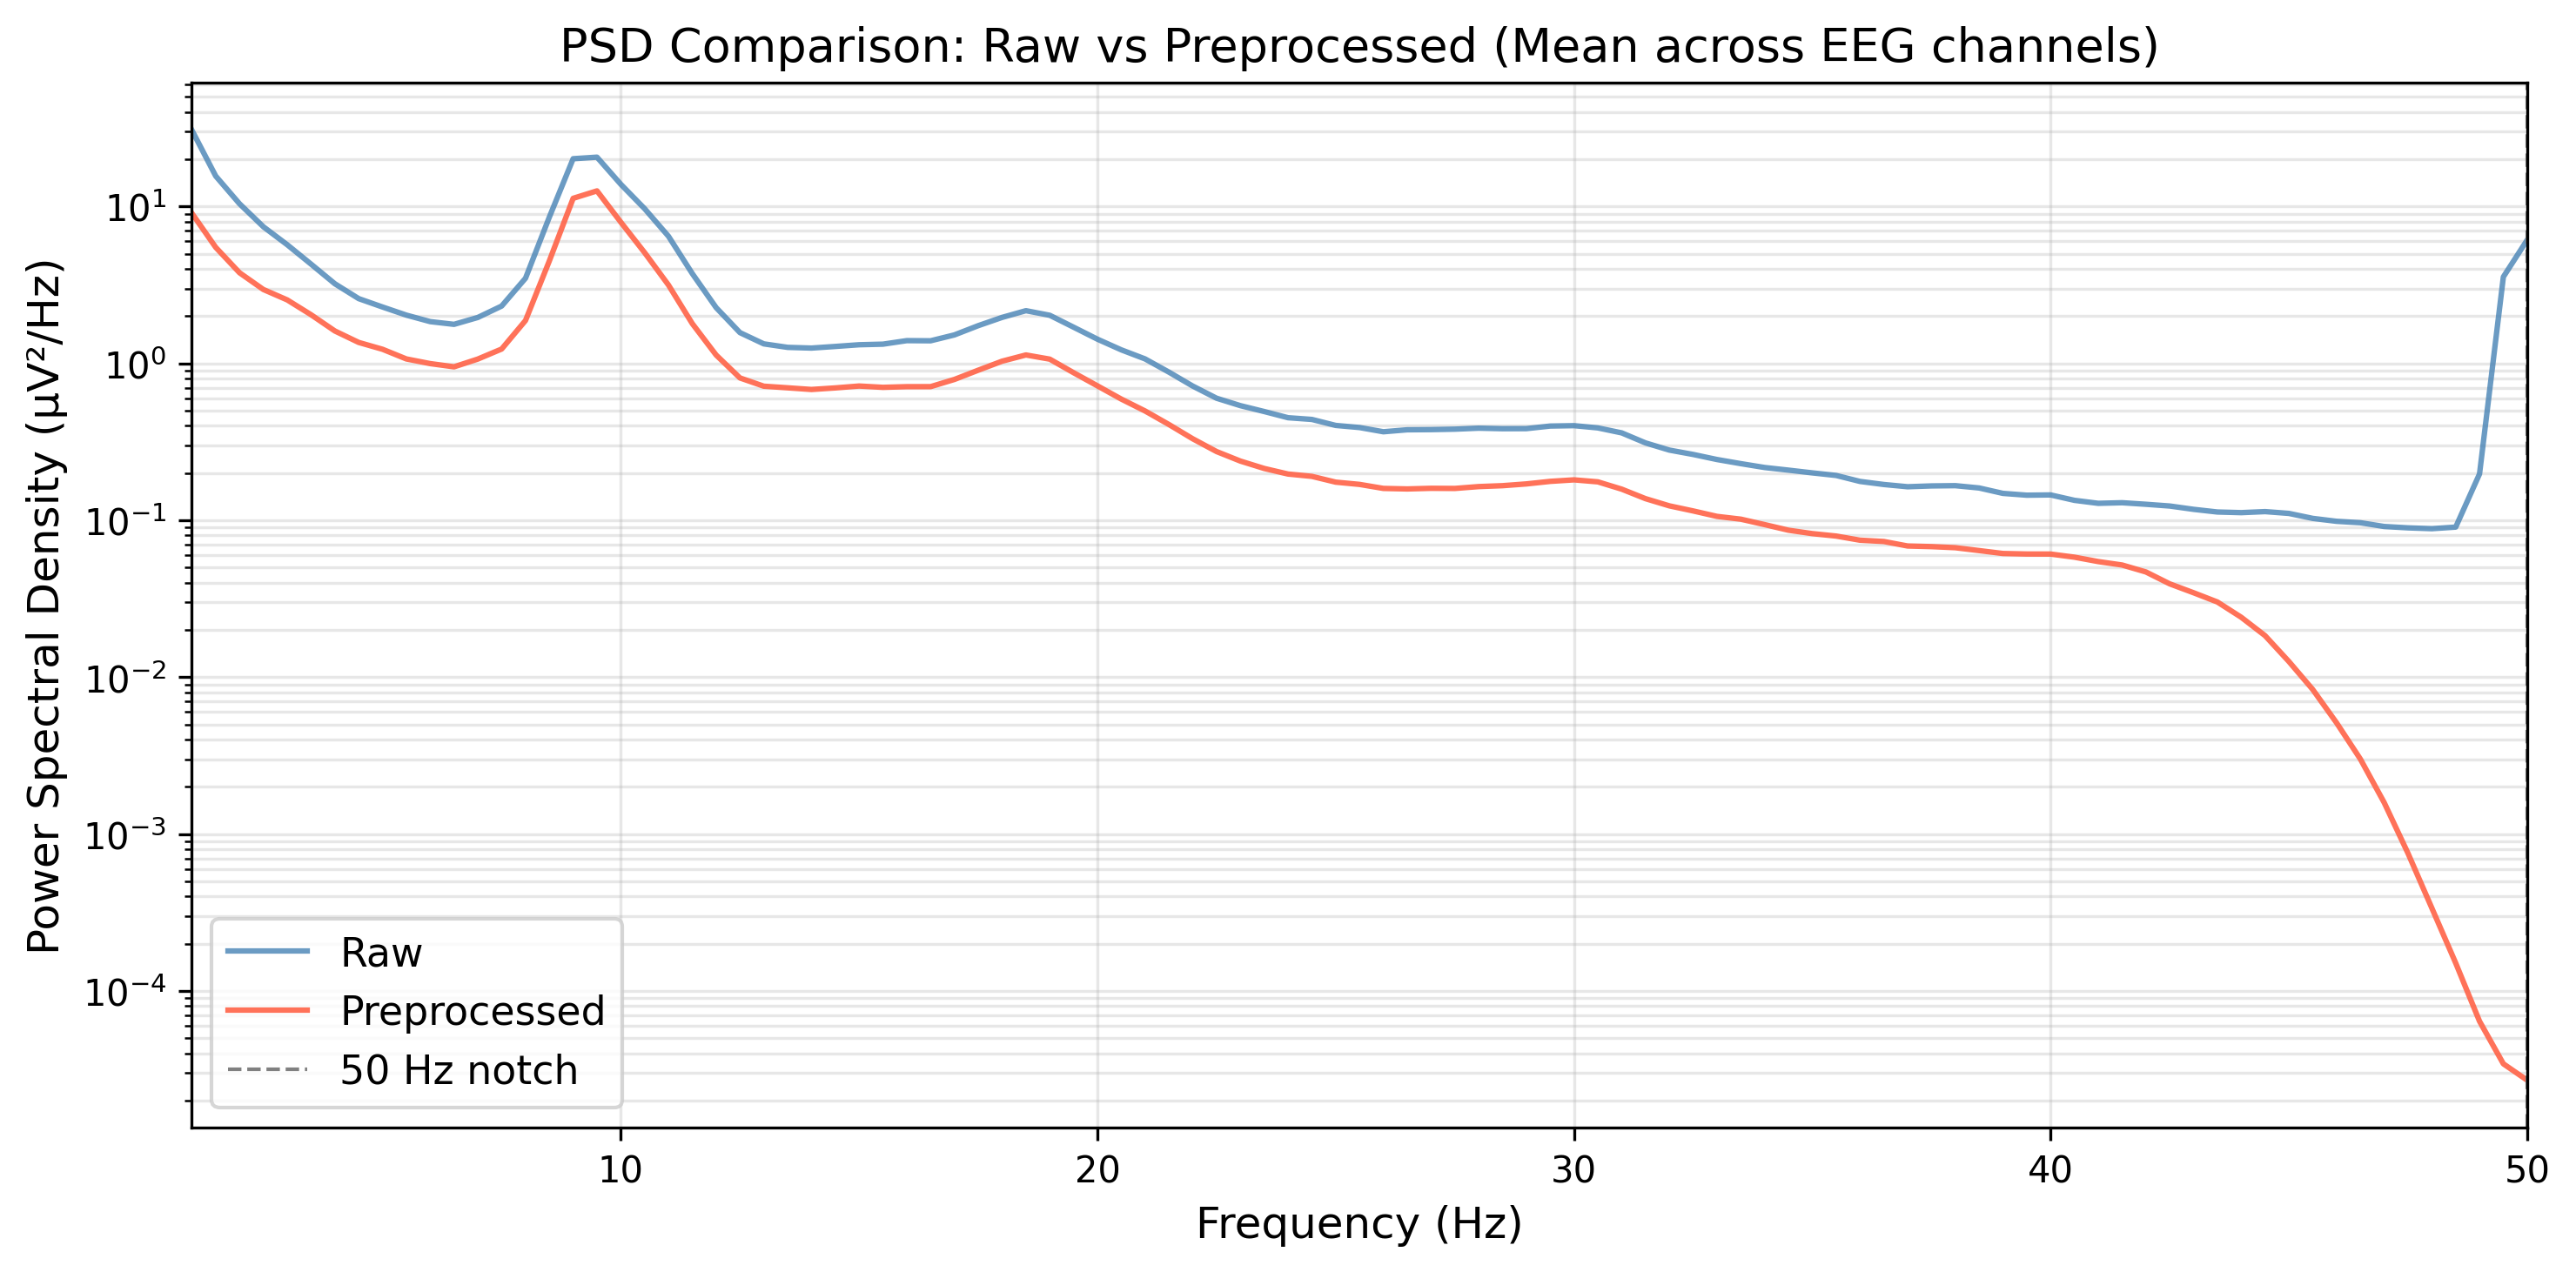
\includegraphics[width=0.82\textwidth]{part1_psd_comparison}
    \caption{Power spectral density comparison between the raw (blue) and
    preprocessed (red) EEG, averaged across all 64 channels. The dashed
    vertical line marks the 50~Hz notch filter.}
    \label{fig:psd}
\end{figure*}

Figure~\ref{fig:psd} shows the PSD comparison. Several observations
stand out. First, the prominent alpha peak around 9--11~Hz is preserved
in both traces, which is expected given the eyes-closed paradigm that
strongly drives alpha oscillations. This confirms that filtering did not
distort physiologically relevant oscillatory activity. Second, there is a
visible notch at 50~Hz in the preprocessed trace, confirming successful
removal of power-line interference. Third, the preprocessed trace shows
attenuated power below 2~Hz (DC drift removal) and above 20~Hz (muscle
artifact and ICA cleaning), while the raw trace shows elevated power in
both bands. The overall downward shift of the preprocessed PSD reflects
the combined removal of artifactual variance, not signal loss.

\begin{figure*}[htbp]
    \centering
    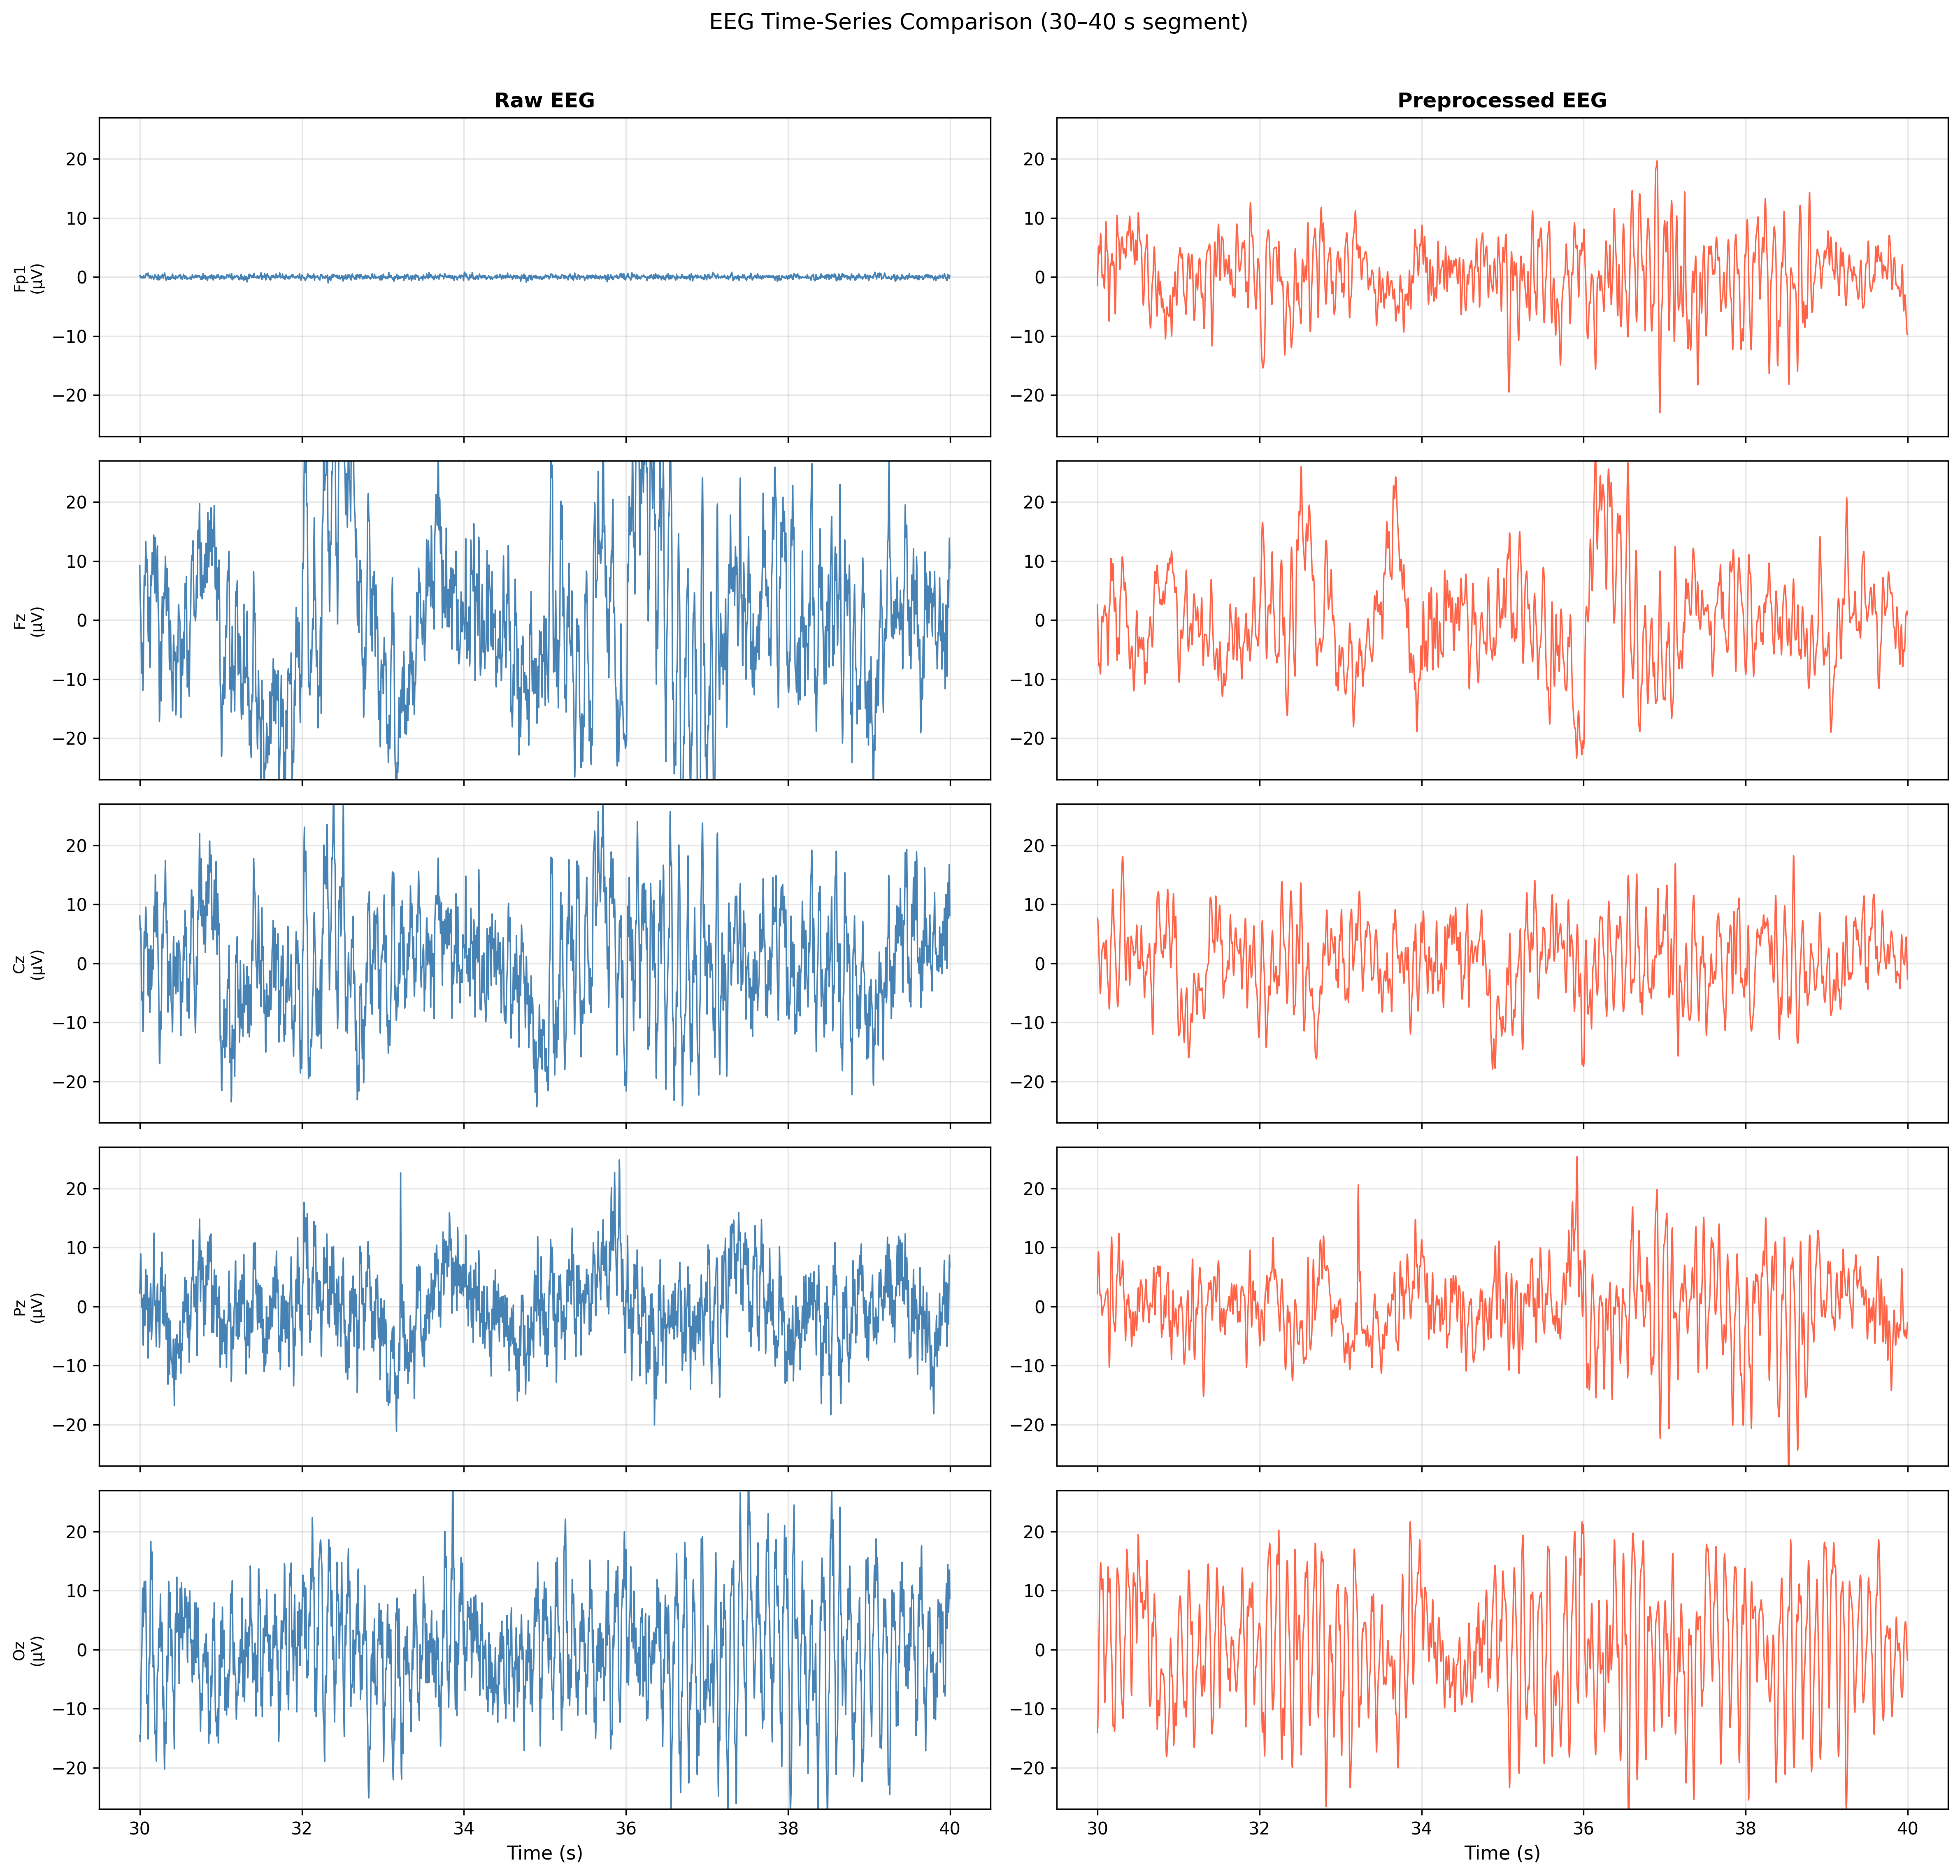
\includegraphics[width=0.88\textwidth]{part1_timeseries_comparison}
    \caption{Ten-second EEG time-series (30--40~s) at five representative
    channels before (blue, left column) and after (red, right column)
    preprocessing. Both columns share the same amplitude scale.}
    \label{fig:timeseries}
\end{figure*}

Figure~\ref{fig:timeseries} shows the time-series comparison. The Fp1
trace in the raw data contains large intermittent transients (eye blinks,
peaking well above 100~$\mu$V) that are completely removed in the
preprocessed trace. Slow drifts visible at Fz and Oz in the raw data are
removed by the high-pass filter, leaving cleaner oscillatory activity.
The Pz channel shows minimal contamination in raw data and looks similar
before and after preprocessing, which is reassuring given that Pz is the
primary channel of interest for P300. The Cz trace shows reduced variance
in the preprocessed version, reflecting muscle artifact removal by ICA.

\begin{figure*}[htbp]
    \centering
    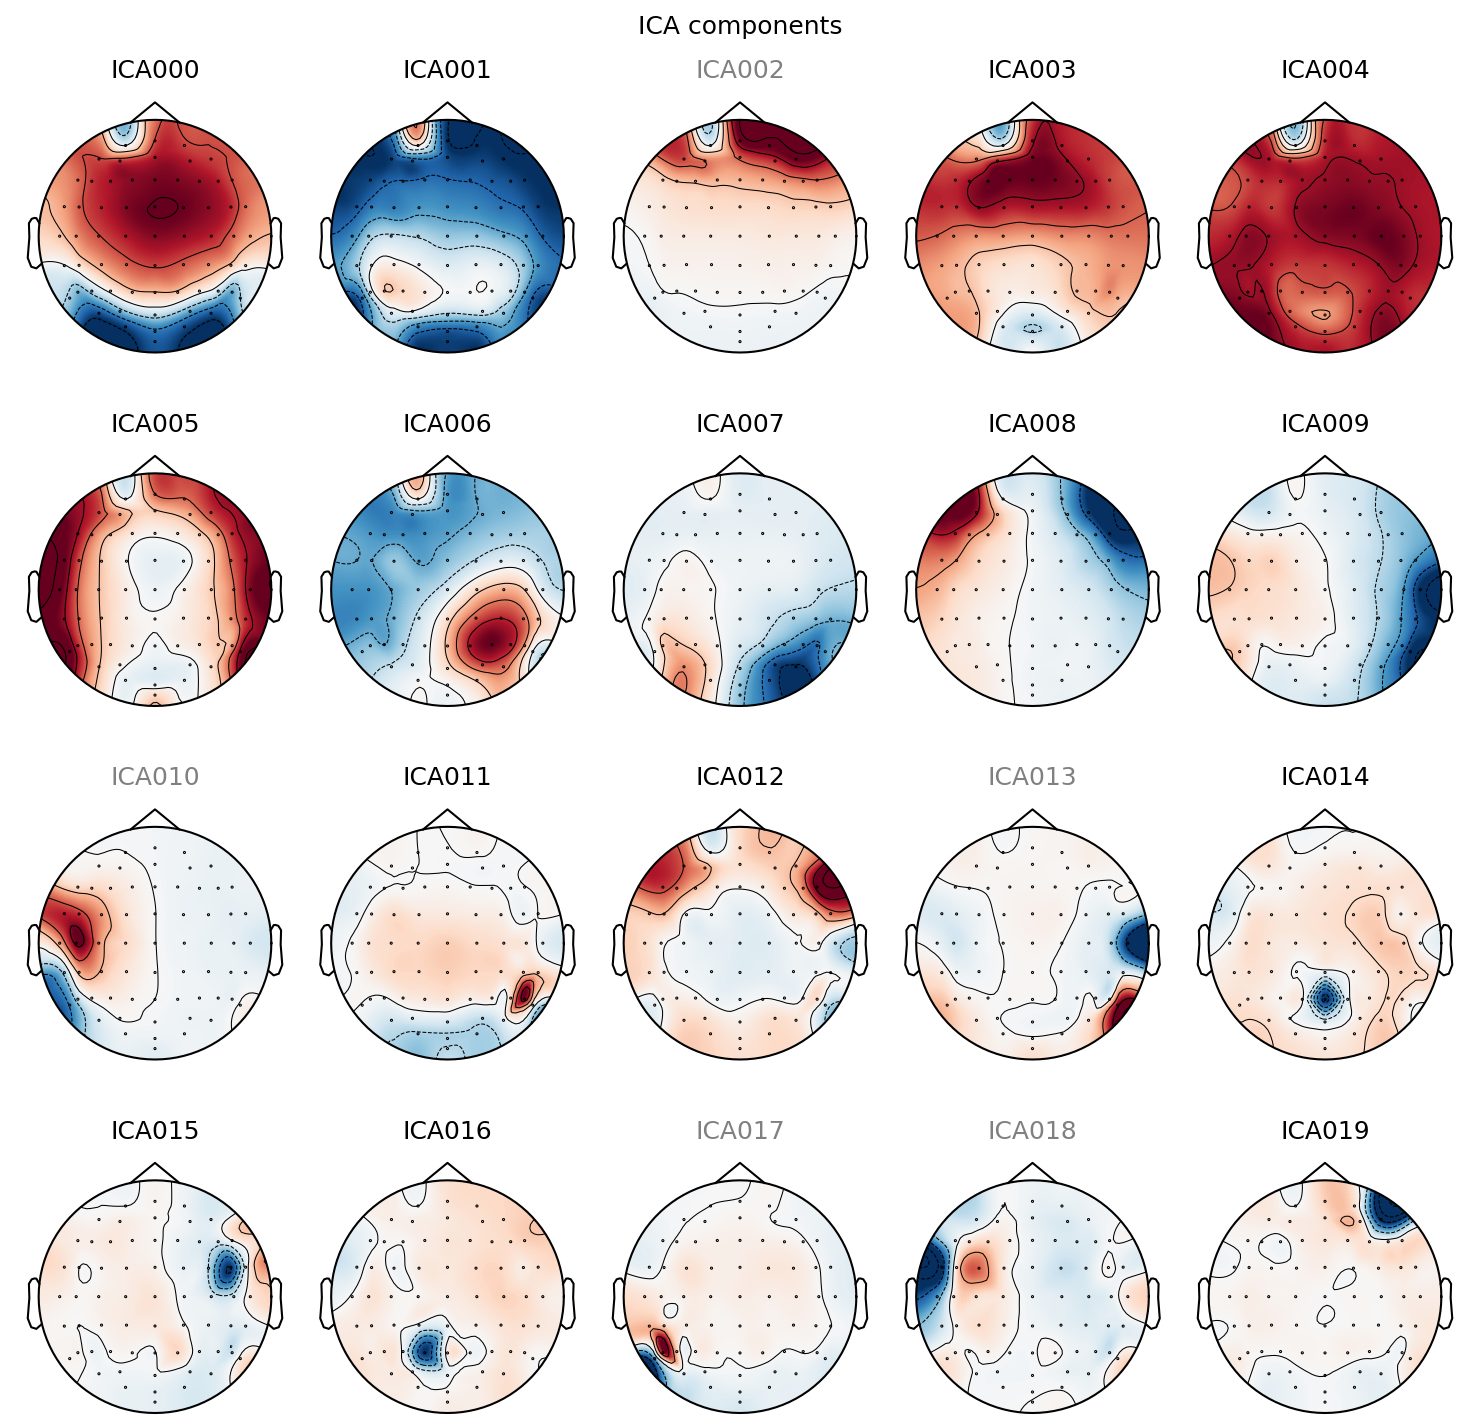
\includegraphics[width=0.88\textwidth]{part1_ica_components}
    \caption{Scalp topographies of the 20 ICA components. Components 2,
    10, 13, 17, and 18 were rejected based on ocular and muscle artifact criteria.}
    \label{fig:ica}
\end{figure*}

Figure~\ref{fig:ica} displays the ICA component topographies. The
removed components are identifiable by their characteristic spatial
patterns: frontal midline/bilateral topography (eye blinks), lateral
frontal dipoles (saccades), and temporal/peripheral focal patterns
(muscle).

\section{Part 2: Epoching and Event-Related Potentials}

\subsection{Research Question}

Does the P300 component (300--500~ms, centro-parietal channels)
differ significantly in mean amplitude across the three stimulus conditions:
standard, oddball, and noise?

\subsection{Null and Alternative Hypotheses}

\textbf{Null hypothesis (H\textsubscript{0}):} There is no difference in
mean P300 amplitude (300--500~ms, channels Pz, CPz, P3, P4, Cz) across
the three stimulus conditions (standard, oddball, noise).

\textbf{Alternative hypothesis (H\textsubscript{A}):} At least one
condition differs significantly from the others in mean P300 amplitude
during the 300--500~ms window.

\subsection{Methodology}

\subsubsection{Segmentation and Baseline Correction}

Events were parsed from the accompanying \texttt{\_events.tsv} file. The
event values \texttt{oddball\_with\_response} and
\texttt{noise\_with\_response} and \texttt{standard\_with\_response} were
collapsed into their respective base condition codes. This preserved all
stimulus events regardless of whether the participant also responded, which
is appropriate for an ERP analysis of stimulus processing rather than
response selection.

Epochs were extracted from $-200$ to $+800$~ms relative to each stimulus
onset. This window provides 200~ms of pre-stimulus baseline and captures
the full P300 waveform including its offset. Baseline correction was
applied by subtracting the mean of the $-200$ to $0$~ms interval from
each epoch, removing pre-stimulus offset differences between trials.
Epochs with peak-to-peak amplitude exceeding 150~$\mu$V in any EEG channel
were rejected to remove residual transient artifacts.

\subsubsection{Averaging}

Epochs were averaged within each condition to obtain evoked responses.
The averages were computed separately for standard, oddball, and noise
conditions.

\subsection{Results}

\subsubsection{Epoch Statistics}

\begin{table}[htbp]
    \centering
    \caption{Epoch counts per condition after preprocessing and rejection.}
    \label{tab:epochs}
    \begin{tabular}{lccc}
        \toprule
        Condition & Events in TSV & Retained & Rejection rate \\
        \midrule
        Standard  & 522 & 518 & 0.8\% \\
        Oddball   & 113 & 112 & 0.9\% \\
        Noise     & 112 & 111 & 0.9\% \\
        \midrule
        Total     & 747 & 741 & 0.8\% \\
        \bottomrule
    \end{tabular}
\end{table}

The rejection rate of 0.8\% across all conditions confirms that the
preprocessing pipeline produced a very clean continuous signal. Only 6
trials were rejected from 747 total events.

\subsubsection{ERP Waveforms}

\begin{figure*}[htbp]
    \centering
    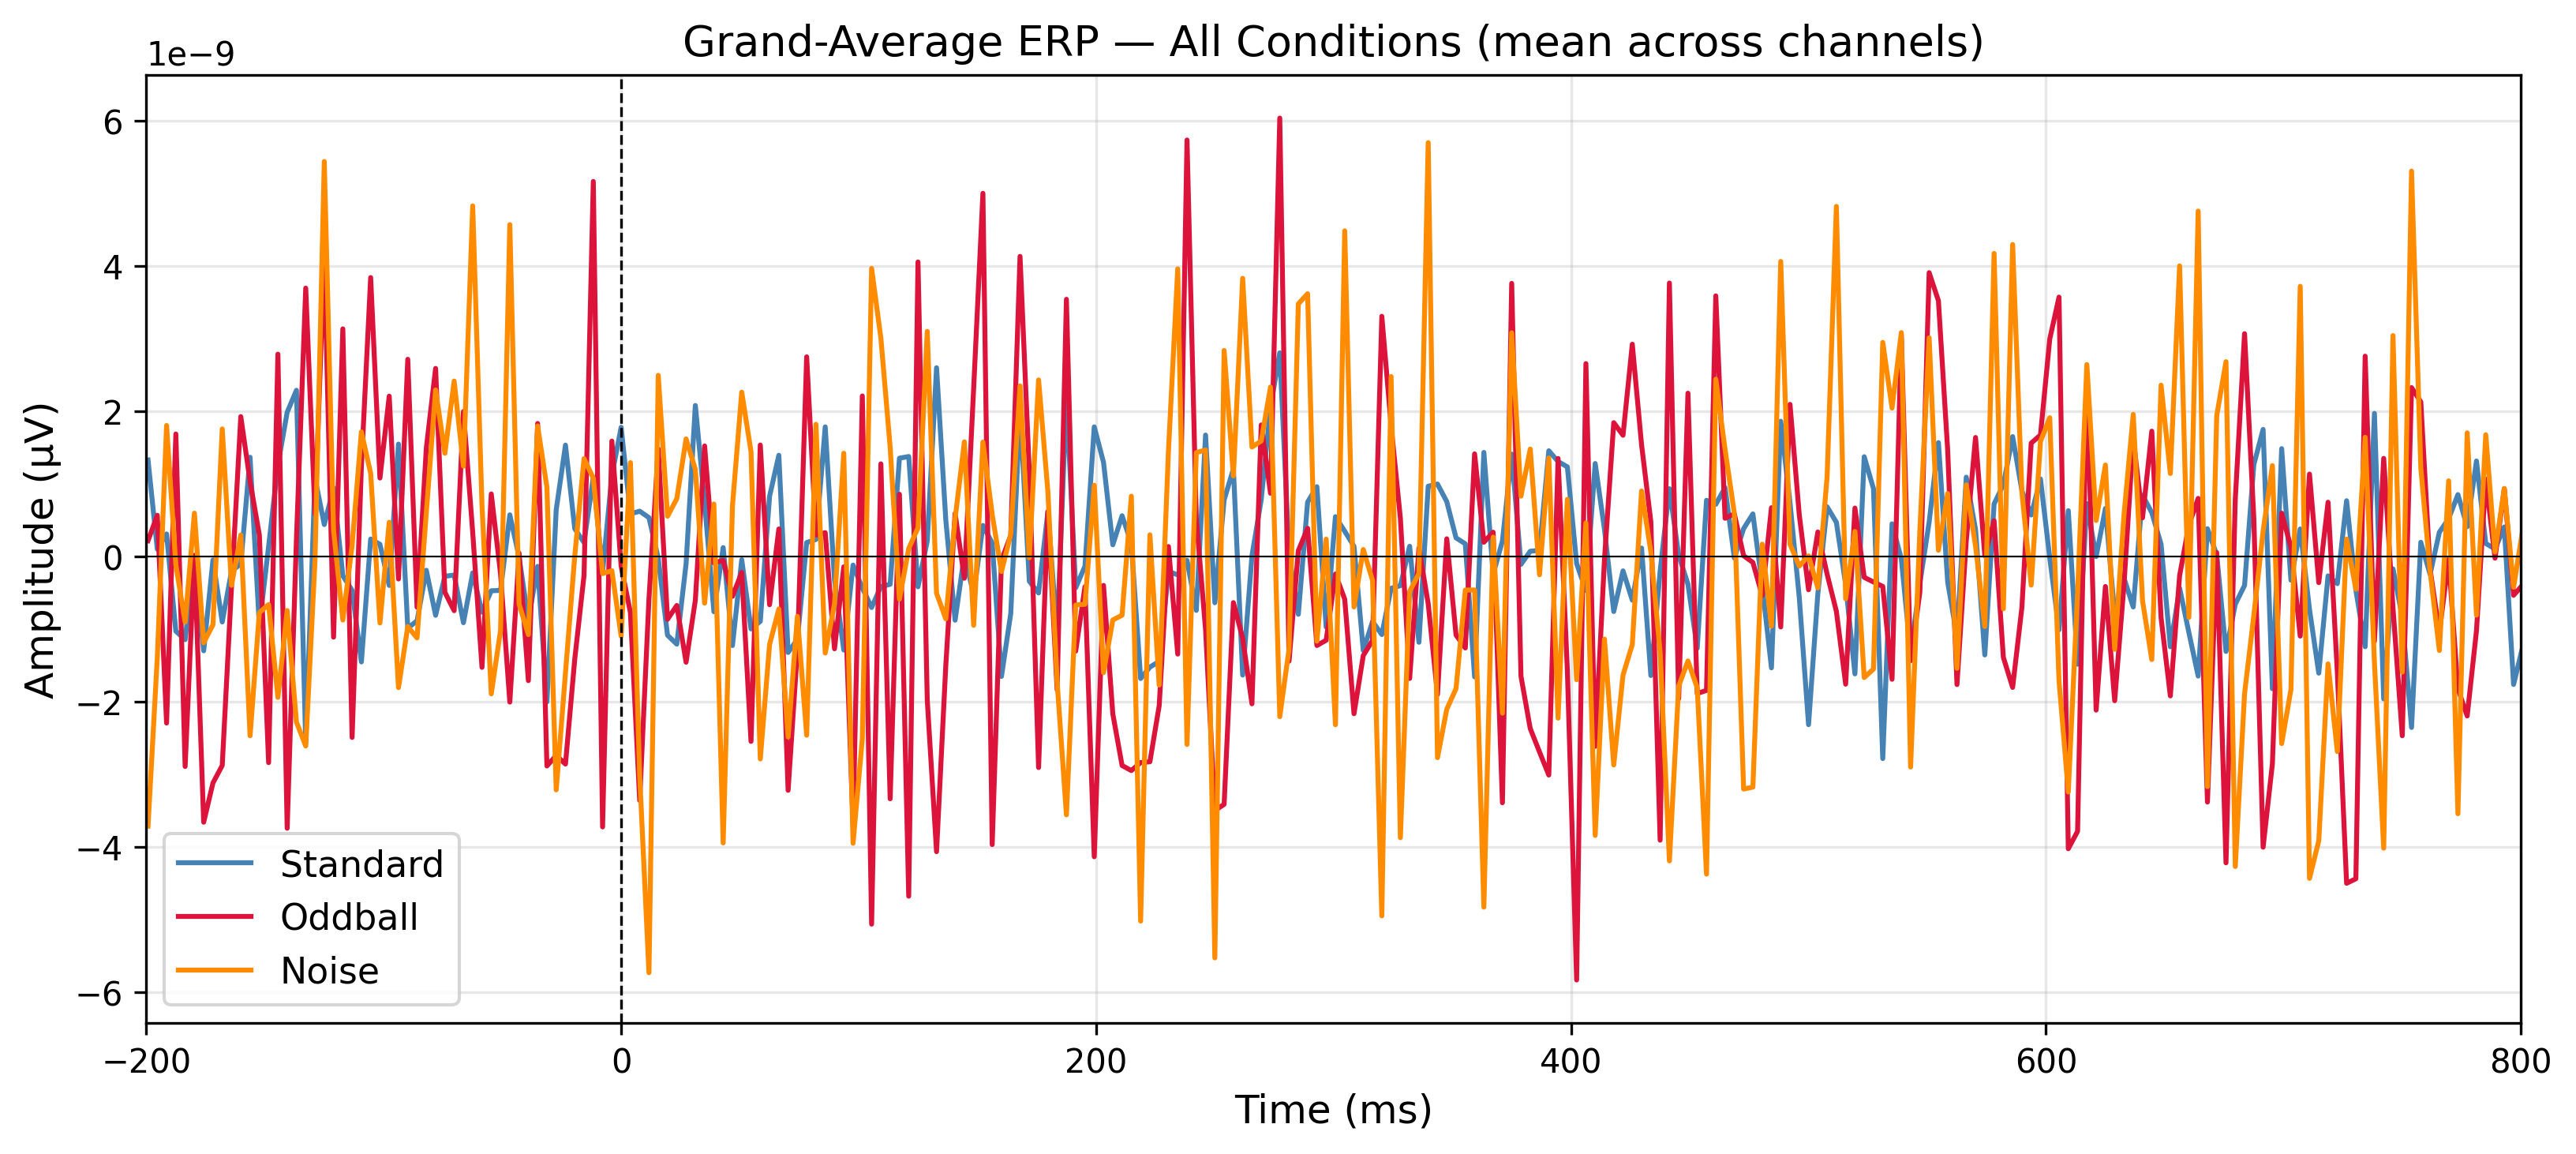
\includegraphics[width=0.82\textwidth]{part2_erp_butterfly_conditions}
    \caption{Grand-average ERP waveforms for all three conditions averaged across all 64 channels.
    The oddball condition (red) shows a prominent positive deflection in the 300--500~ms window consistent with P300.}
    \label{fig:butterfly}
\end{figure*}

Figure~\ref{fig:butterfly} shows the mean ERP across all channels for
each condition. The oddball condition produces a clearly distinguishable
large positive component between 200 and 600~ms. The noise condition shows
a modest positive deflection while the standard remains near zero throughout
the post-stimulus window, consistent with the expected outcome of the
three-stimulus paradigm.

\begin{figure*}[htbp]
    \centering
    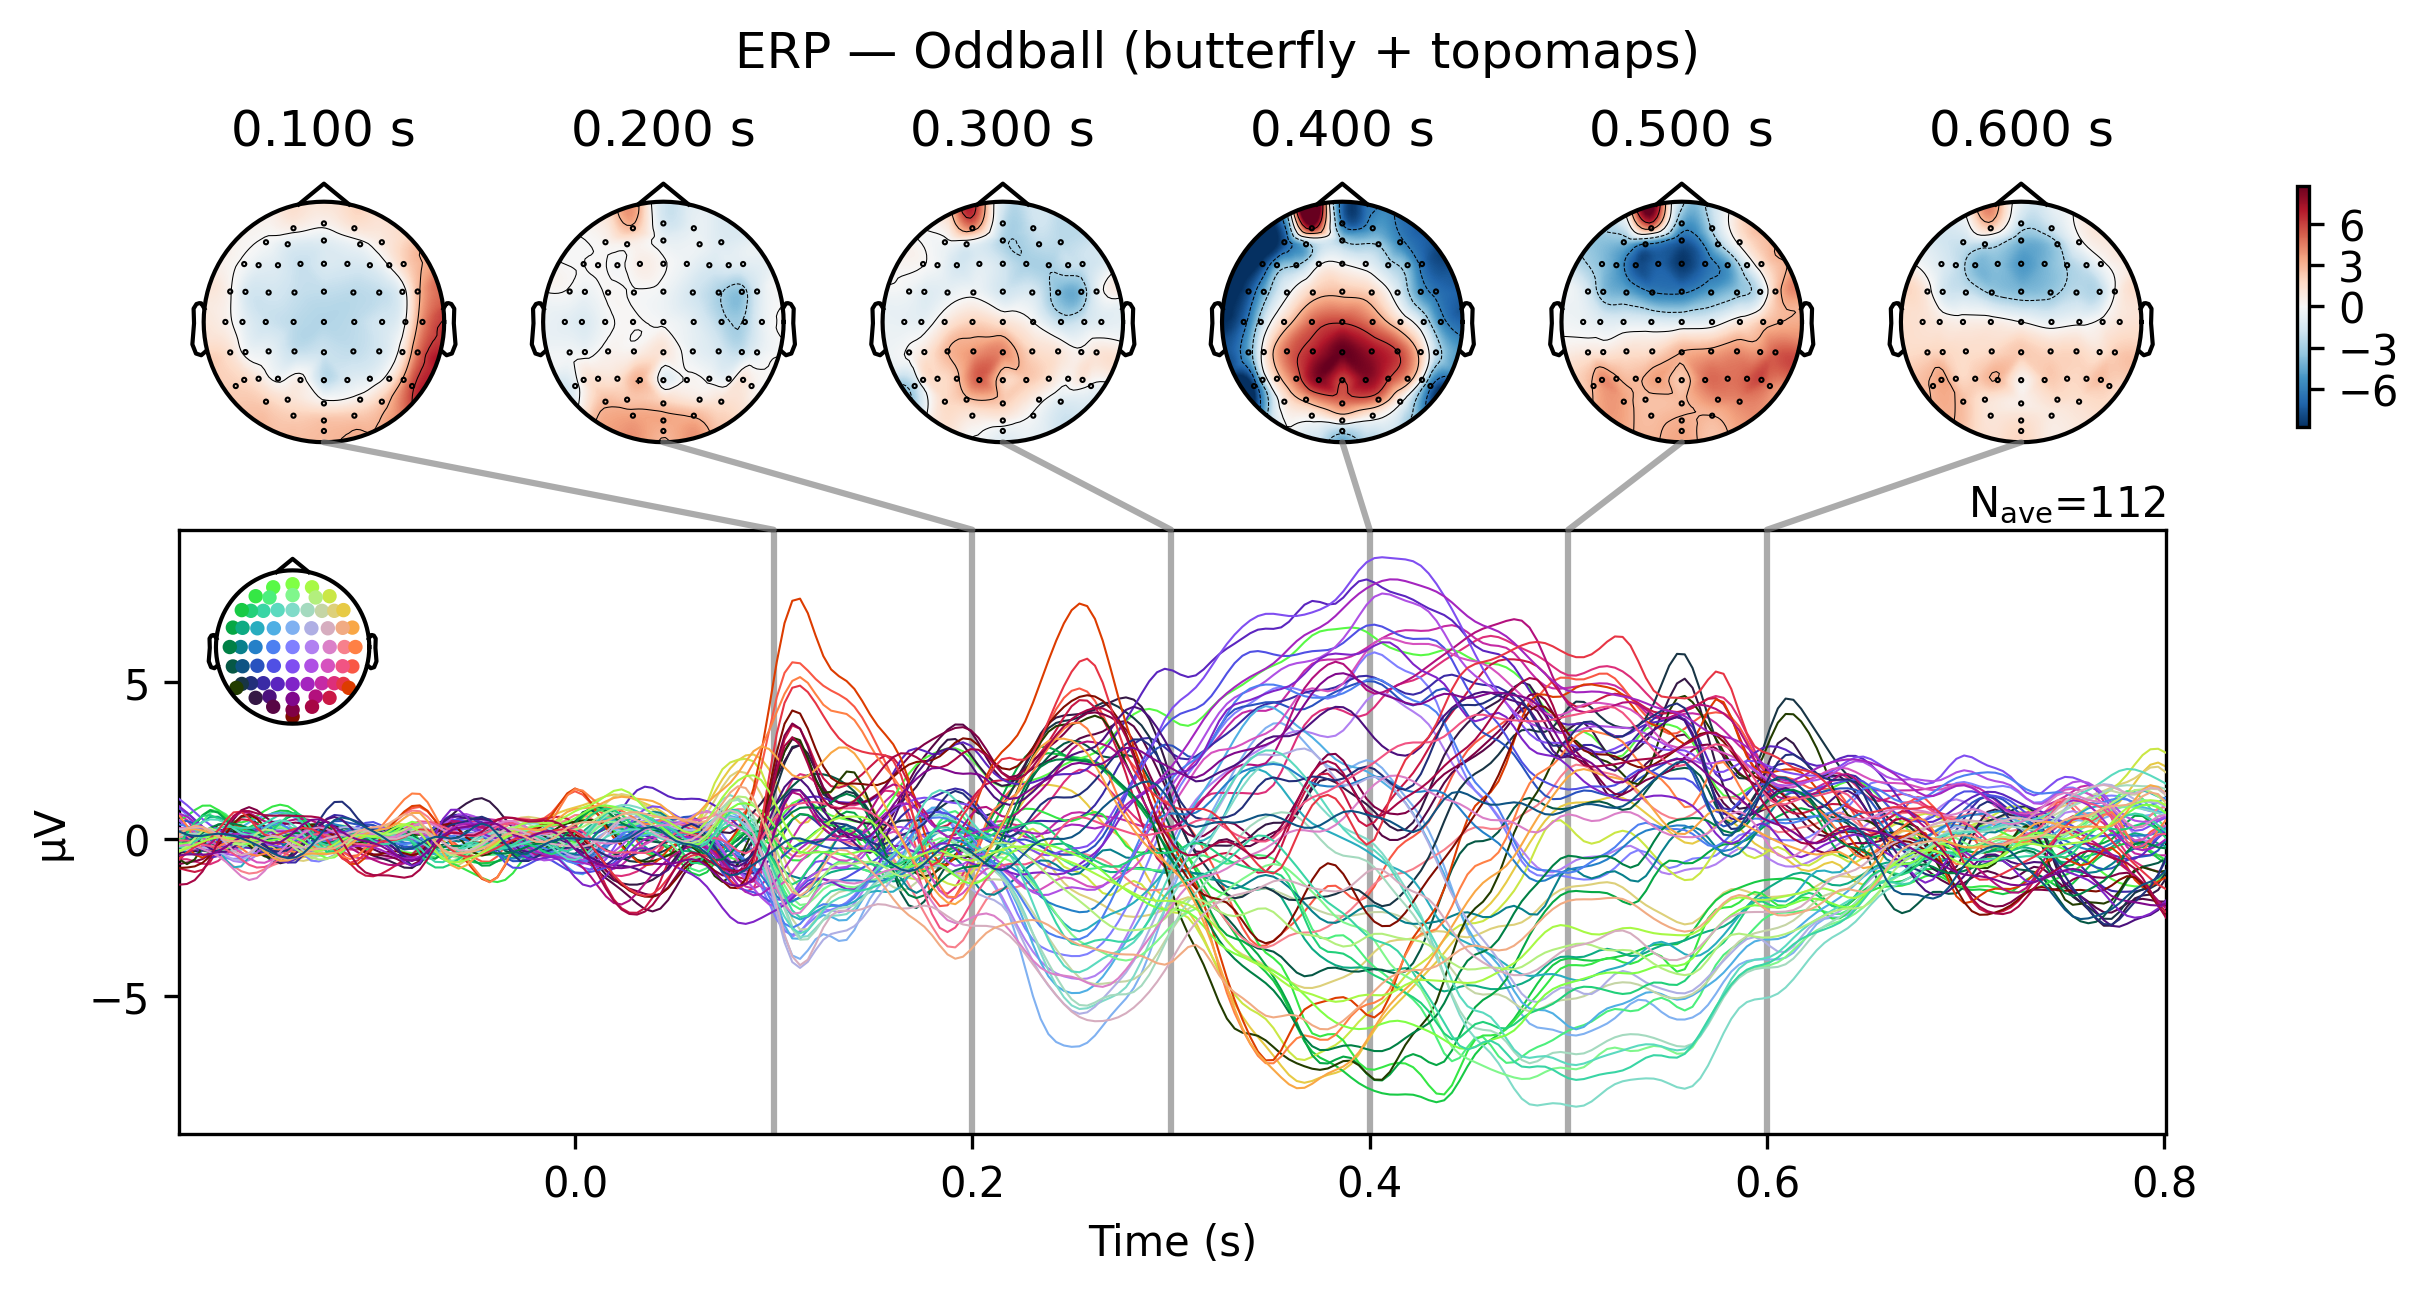
\includegraphics[width=0.88\textwidth]{part2_erp_joint_oddball}
    \caption{Butterfly plot and scalp topographies at selected latencies for the oddball condition.
    Each line is one EEG channel. Topomaps at 300, 400, and 500~ms show the characteristic
    centro-parietal P300 distribution.}
    \label{fig:joint_oddball}
\end{figure*}

Figure~\ref{fig:joint_oddball} shows the channel-by-channel butterfly
plot for the oddball condition along with topographic snapshots at
100, 200, 300, 400, 500, and 600~ms. At 300--400~ms, a strong, broadly
distributed centro-parietal positivity is apparent, with the maximum
near Pz and CPz. This distribution is characteristic of the P3b subcomponent,
which reflects target detection and working memory context updating
\citep{Donchin1988, Polich2007}.

\begin{figure*}[htbp]
    \centering
    \begin{minipage}[t]{0.56\textwidth}
        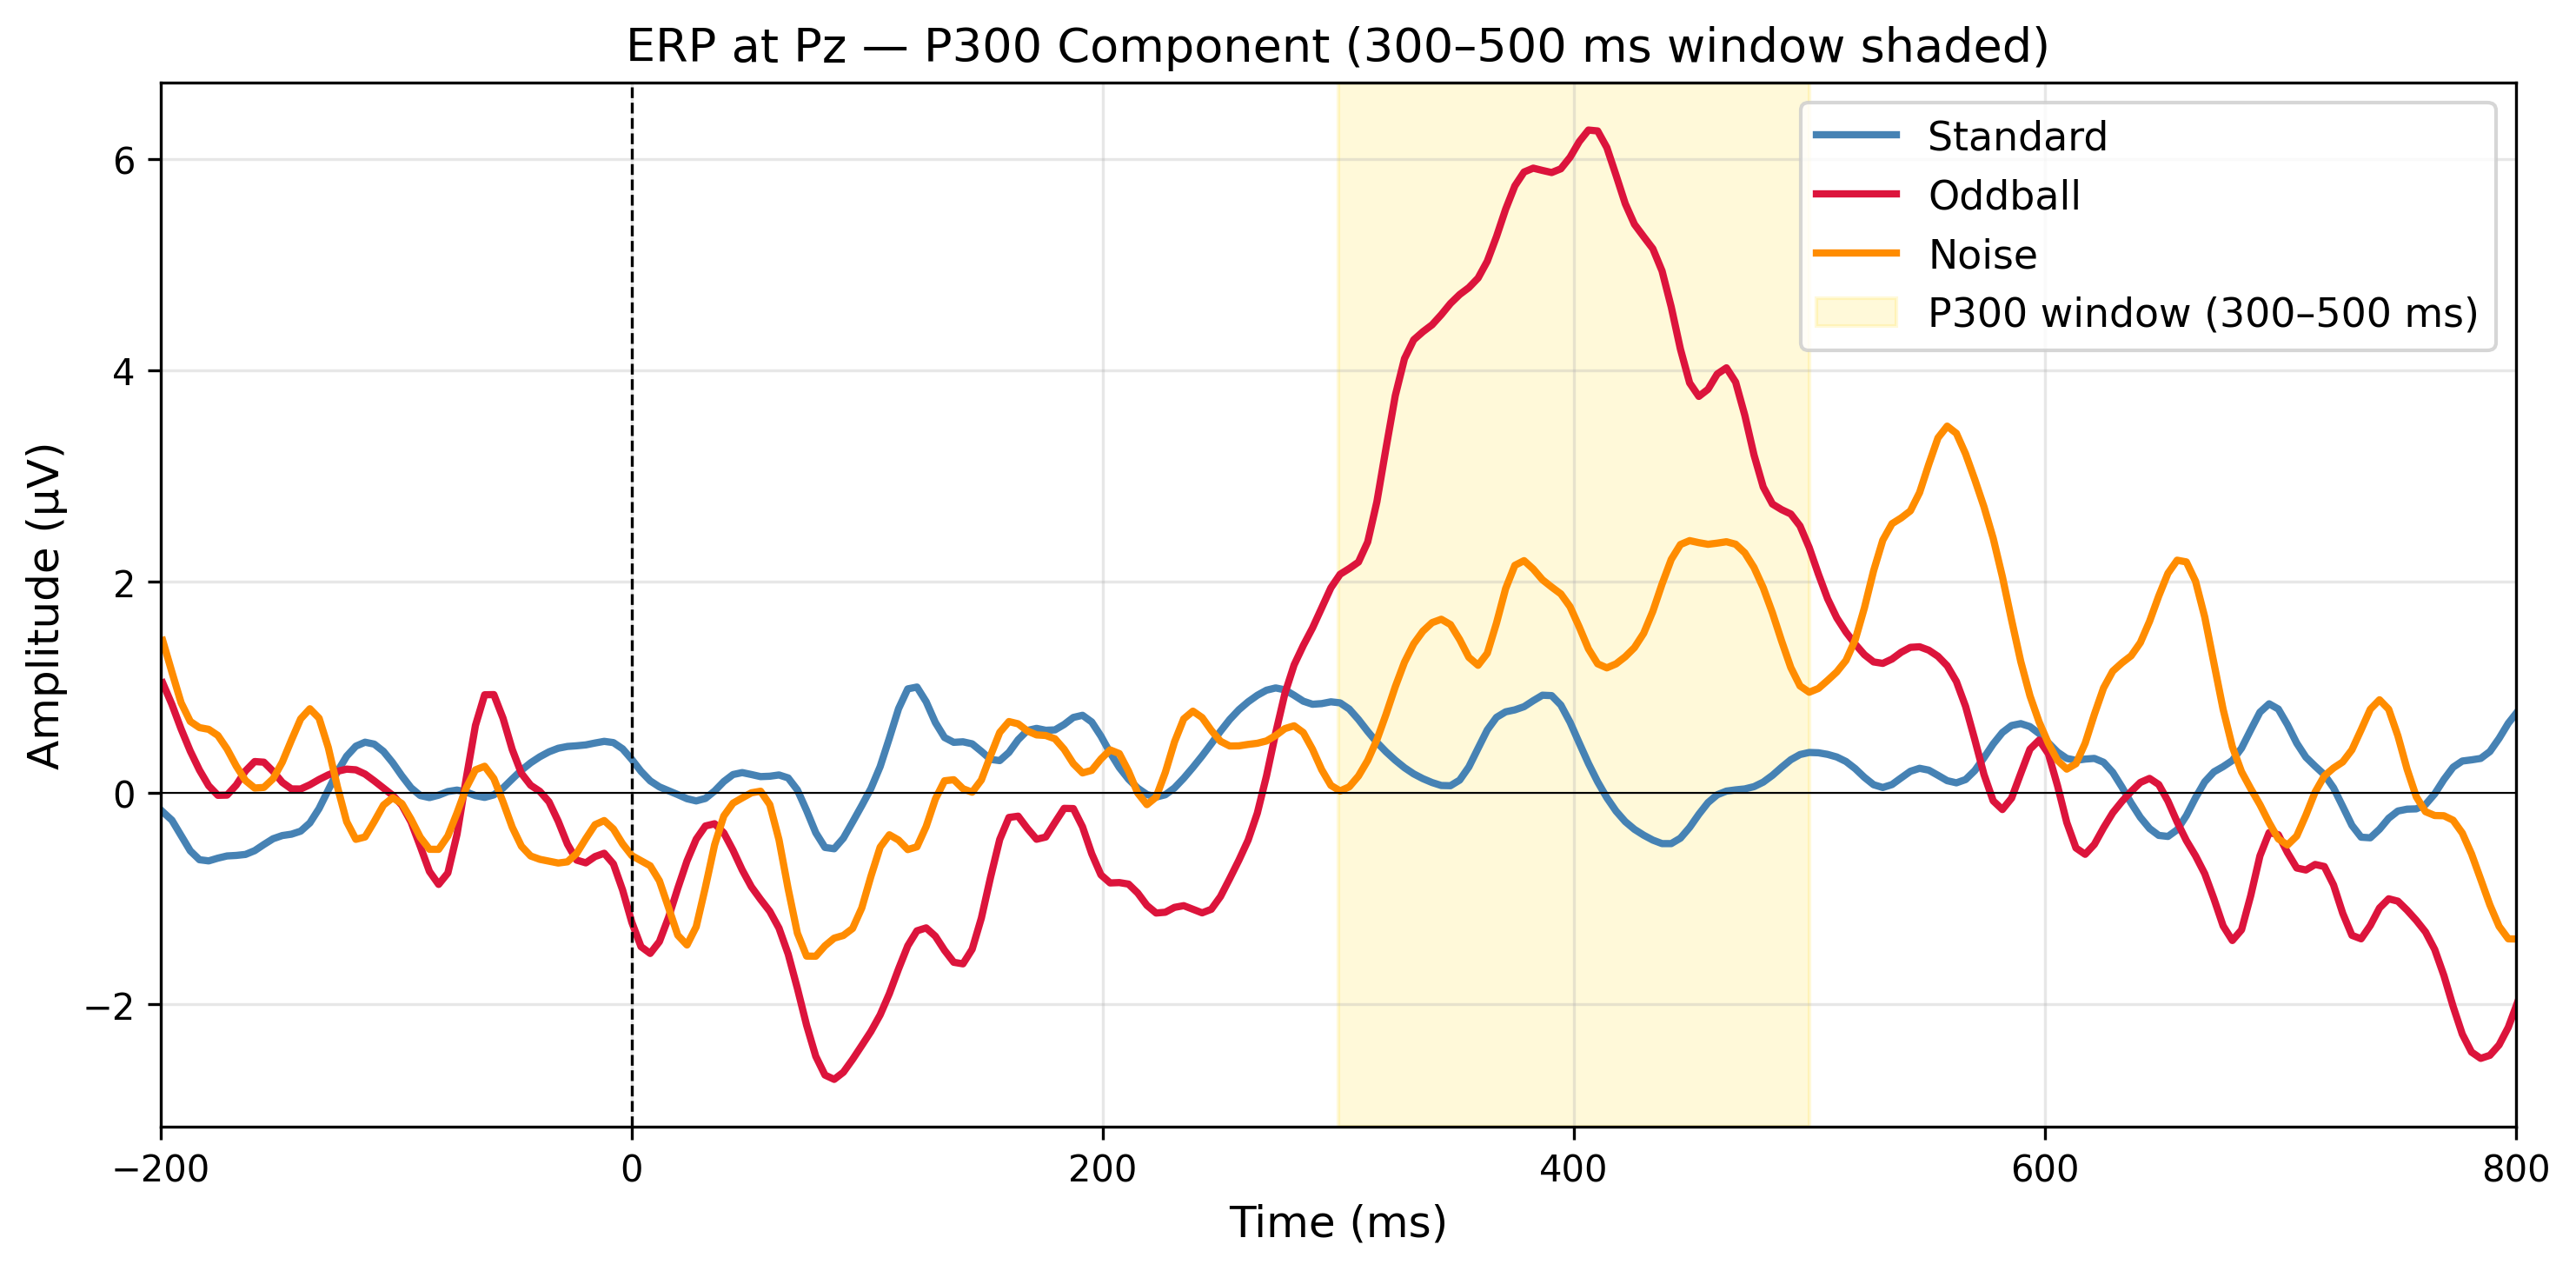
\includegraphics[width=\linewidth]{part2_erp_Pz_P300}
        \caption{ERP at Pz for all three conditions. Shaded region (300--500~ms) marks the
        P300 window. Oddball peaks at 406.2~ms, $M = +4.66\ \mu$V.}
        \label{fig:pz_p300}
    \end{minipage}\hfill
    \begin{minipage}[t]{0.40\textwidth}
        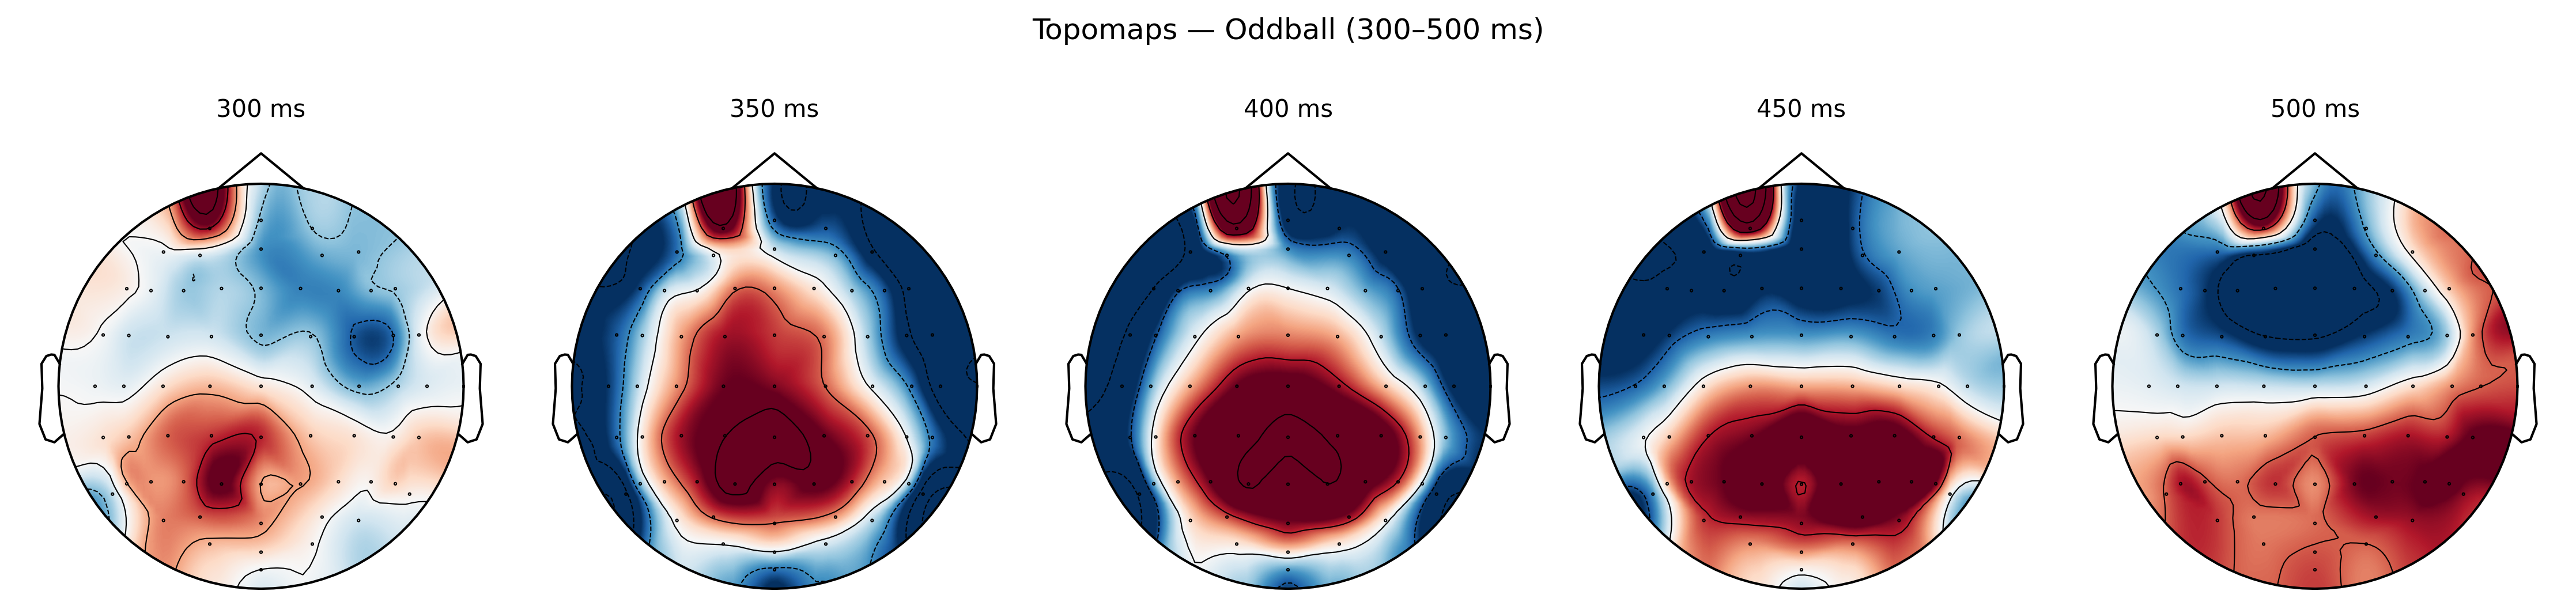
\includegraphics[width=\linewidth]{part2_erp_topomap_oddball}
        \caption{Topomaps at 300, 350, 400, 450, and 500~ms for the oddball condition.
        The centro-parietal maximum peaks around 400~ms.}
        \label{fig:topo_oddball}
    \end{minipage}
\end{figure*}

Figure~\ref{fig:pz_p300} shows the single-channel ERP at Pz. The three
conditions diverge clearly after approximately 250~ms. The oddball waveform
peaks at \textbf{406.2~ms}, well within the established 300--600~ms range
for auditory P3b \citep{Polich2007}. The noise condition shows a smaller
positive deflection that peaks earlier (around 300--350~ms), consistent
with the P3a novelty component rather than the target-specific P3b. The
standard condition remains close to baseline throughout the window.

Figure~\ref{fig:topo_oddball} shows that the P300 topography for the
oddball condition is maximal at centro-parietal midline sites (Pz, CPz)
and remains stable across the 300--500~ms window, which is the hallmark
of the P3b component.

\subsubsection{Statistical Analysis}

Mean amplitude was extracted for each epoch within the 300--500~ms window
and averaged across the five centro-parietal channels of interest (Pz,
CPz, P3, P4, Cz). A one-way independent ANOVA was used to test for
differences across conditions, followed by Bonferroni-corrected pairwise
independent-samples $t$-tests. Effect sizes are reported as Cohen's $d$.

\begin{table}[htbp]
    \centering
    \caption{Descriptive statistics for P300 mean amplitude (300--500~ms,
    channels Pz, CPz, P3, P4, Cz).}
    \label{tab:descriptive}
    \begin{tabular}{lcccc}
        \toprule
        Condition & $n$ & $M$ ($\mu$V) & $SD$ & $SEM$ \\
        \midrule
        Standard  & 518 & $+0.231$ & 2.863 & 0.126 \\
        Oddball   & 112 & $+4.658$ & 3.170 & 0.300 \\
        Noise     & 111 & $+1.081$ & 3.067 & 0.291 \\
        \bottomrule
    \end{tabular}
\end{table}

\begin{figure}[htbp]
    \centering
    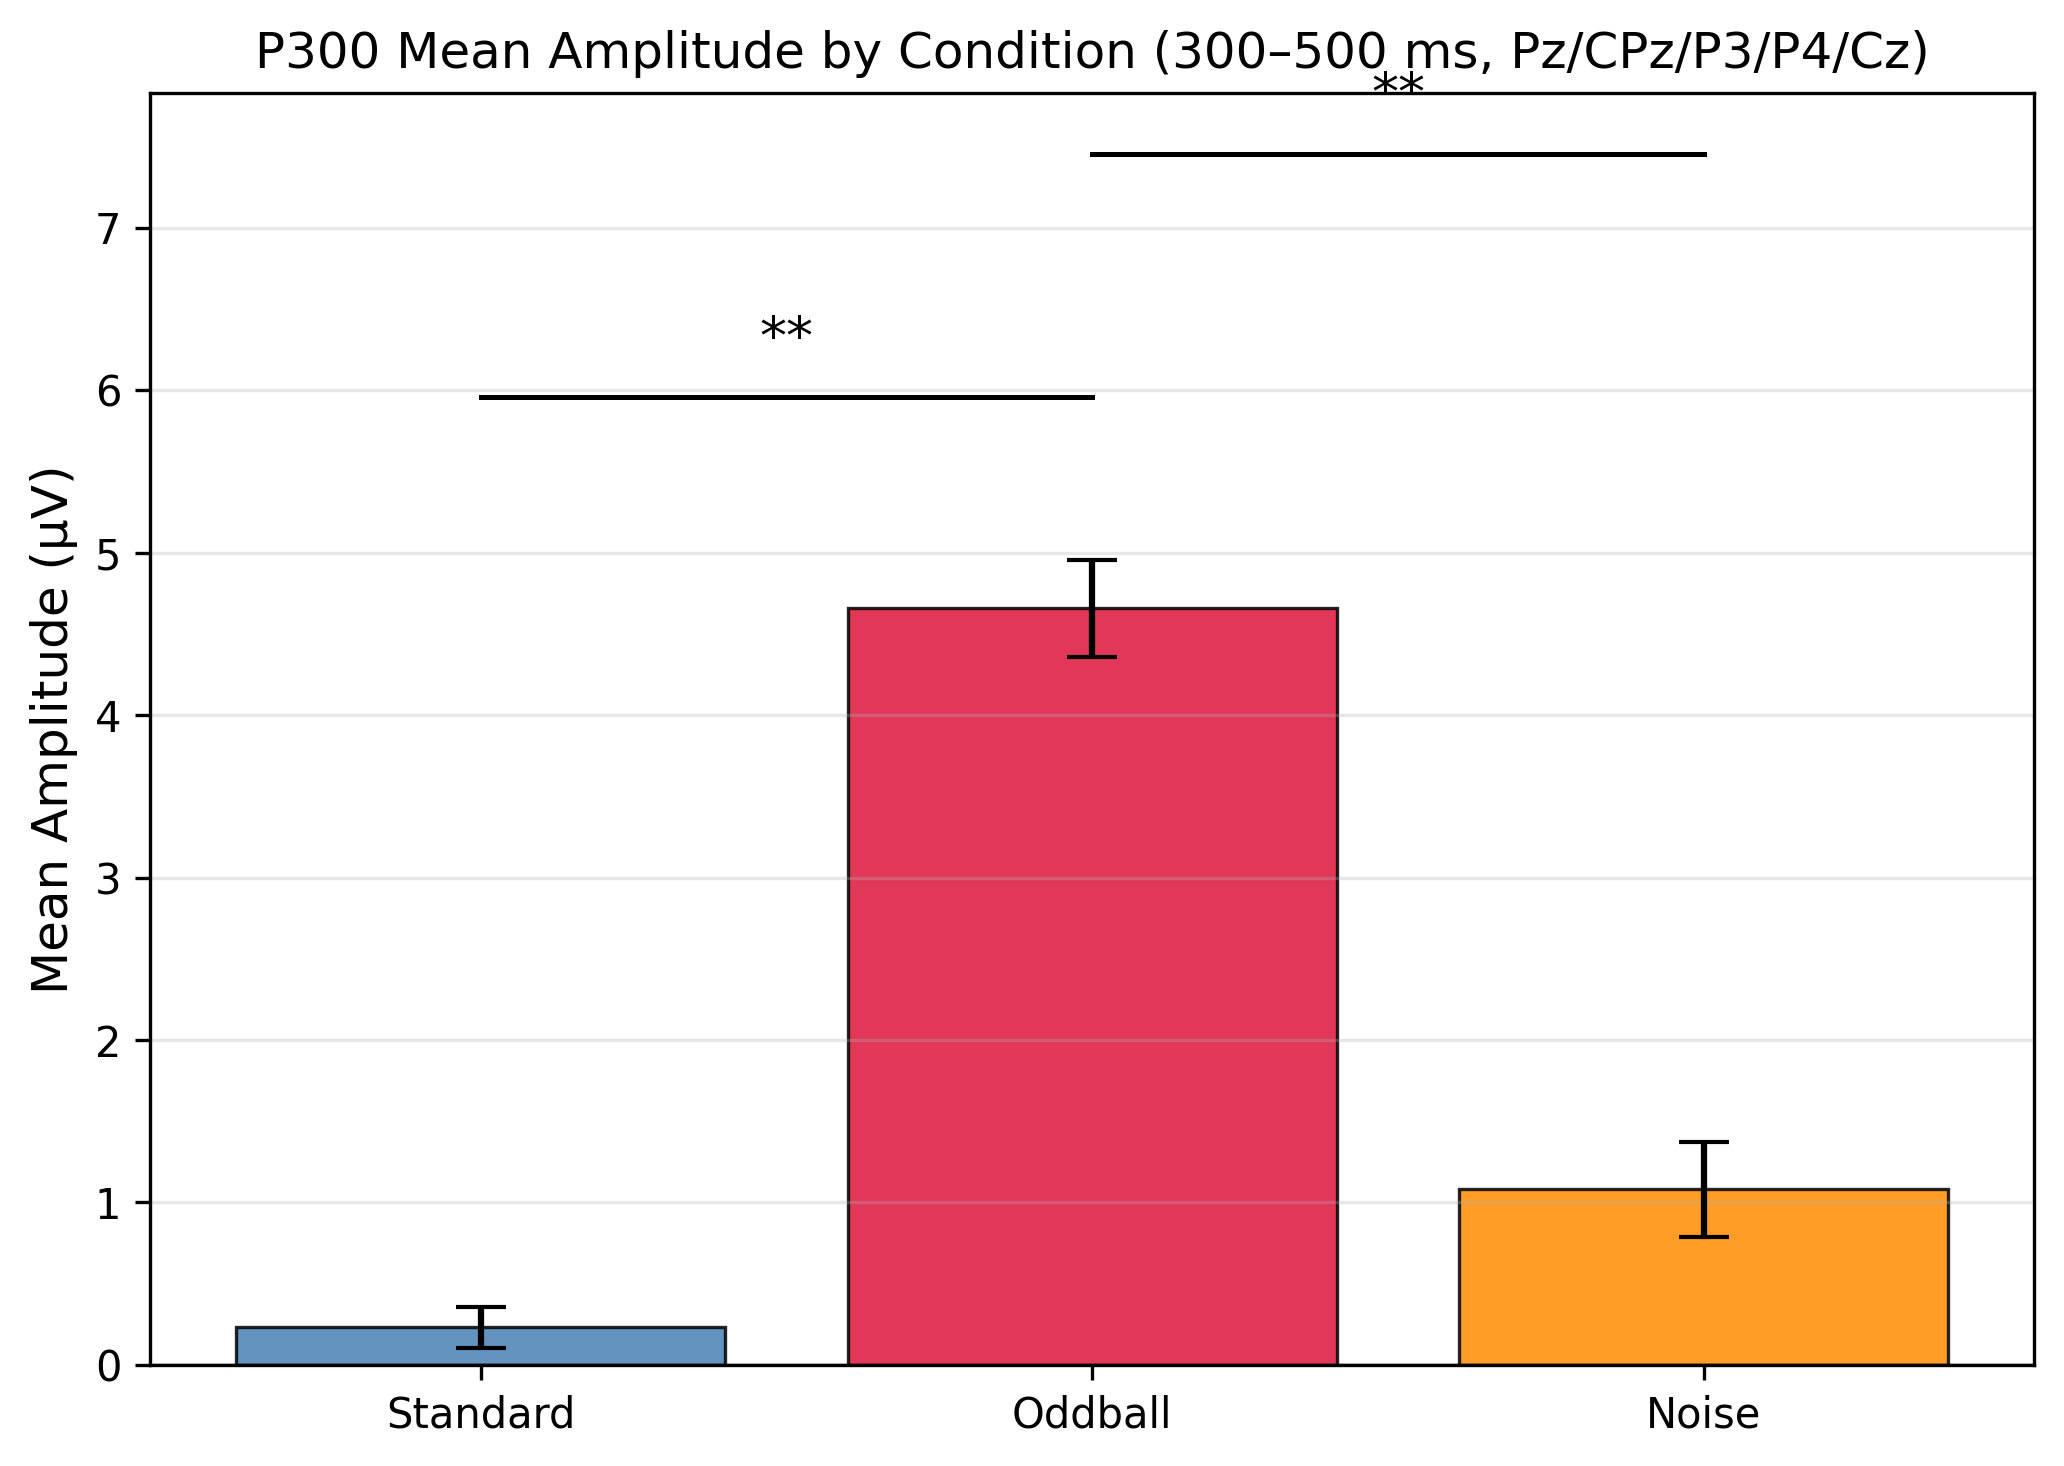
\includegraphics[width=\linewidth]{part2_P300_amplitude_barplot}
    \caption{Mean P300 amplitude ($\pm$SEM) by condition. Asterisks mark
    significant differences after Bonferroni correction ($\alpha = .017$).}
    \label{fig:barplot}
\end{figure}

A one-way ANOVA revealed a significant main effect of stimulus condition on
P300 mean amplitude, $F(2, 738) = 103.86$, $p < .001$. Post-hoc pairwise
comparisons with Bonferroni correction ($\alpha = .017$) showed that the
oddball condition produced significantly larger P300 amplitude than both
the standard condition, $t(628) = 14.53$, $p < .001$, $d = 1.46$, and the
noise condition, $t(221) = 8.53$, $p < .001$, $d = 1.14$. The standard and
noise conditions also differed significantly, $t(627) = -2.80$, $p = .016$.

\subsection{Discussion}

The results provide strong evidence in support of the alternative
hypothesis. The oddball condition elicited a significantly larger P300
than both non-target conditions, with large effect sizes ($d > 1.0$) for
both comparisons. A peak latency of 406.2~ms at Pz falls squarely within
the expected range for auditory P3b in a simple oddball paradigm
\citep{Verleger1997, Polich2007}.

The amplitude ordering across conditions (oddball $>$ noise $>$ standard)
is consistent with the theoretical framework proposed by \citet{Polich2007},
where P300 amplitude reflects the probability-weighted allocation of
attentional resources. The oddball required a motor response
(button press), engaging both the P3b target-detection mechanism and
working memory updating processes. The noise distractor elicited a
smaller, earlier positivity, more consistent with the P3a component
driven by novelty and involuntary attention capture \citep{Polich2007}.
The standard tone, being frequent and task-irrelevant, produced minimal
neural response after 200~ms.

The very high epoch retention rate (99.2\%) and the clean waveform
morphology confirm that the preprocessing pipeline was effective without
over-cleaning the data.

\section{Part 3: Reference Comparison and Topographic Analysis}

\subsection{Research Question}

How does the choice of EEG reference affect the scalp topography and
amplitude of the P300 ERP component, and which reference provides the
most accurate representation of the occipito-temporal neural generators?

\subsection{Null and Alternative Hypotheses}

\textbf{Null hypothesis (H\textsubscript{0}):} The choice of reference
electrode does not significantly affect the scalp topography or the
estimated amplitude of the P300 component at Pz.

\textbf{Alternative hypothesis (H\textsubscript{A}):} Different reference
choices produce systematically different P300 amplitude estimates and
topographic distributions, with the differences attributable to the
reference electrode's own signal contribution.

\subsection{Methodology}

The ICA-cleaned data (prior to any re-referencing) was loaded and five
reference schemes were applied independently:

\begin{enumerate}\setlength{\itemsep}{1pt}\setlength{\parskip}{0pt}
    \item \textbf{Average reference}: mean of all 64 channels subtracted from each channel.
    \item \textbf{Cz reference}: Cz subtracted from all channels (vertex reference).
    \item \textbf{Linked mastoids (TP7+TP8)}: mean of bilateral mastoid electrodes.
    \item \textbf{Fpz reference}: Fpz as a proxy for the nasion site.
    \item \textbf{No re-reference (CMS/DRL)}: original Biosemi offset retained without offline re-referencing.
\end{enumerate}

For each reference, the data were epoched using the same parameters as
Part 2 ($-200$ to $+800$~ms, baseline $-200$ to $0$~ms, 150~$\mu$V
rejection), and the oddball evoked response was computed. The P300 peak
latency at Pz was determined from the average-reference evoked response
within the 250--550~ms window and used as a common reference point for
topographic comparison across all schemes.

\subsection{Results}

\subsubsection{P300 Amplitude and Peak Latency}

The P300 peak latency at Pz under average reference was \textbf{406.2~ms}.
Table~\ref{tab:reference} summarises the mean amplitude (300--500~ms) and
peak latency at Pz for each reference scheme.

\begin{table}[htbp]
    \centering
    \caption{P300 mean amplitude (300--500~ms) and peak latency at Pz under
    five reference schemes, oddball condition.}
    \label{tab:reference}
    \begin{tabular}{lcc}
        \toprule
        Reference Scheme & Mean amplitude ($\mu$V) & Peak latency (ms) \\
        \midrule
        Average reference    & $+4.384$ & 406.2 \\
        Cz reference         & $+1.280$ & 476.6 \\
        Linked mastoids      & $+5.279$ & 398.4 \\
        Fpz (nasion proxy)   & $+9.471$ & 406.2 \\
        No re-reference      & $-1.013$ & 250.0 \\
        \bottomrule
    \end{tabular}
\end{table}

\subsubsection{Scalp Topographies}

\begin{figure*}[htbp]
    \centering
    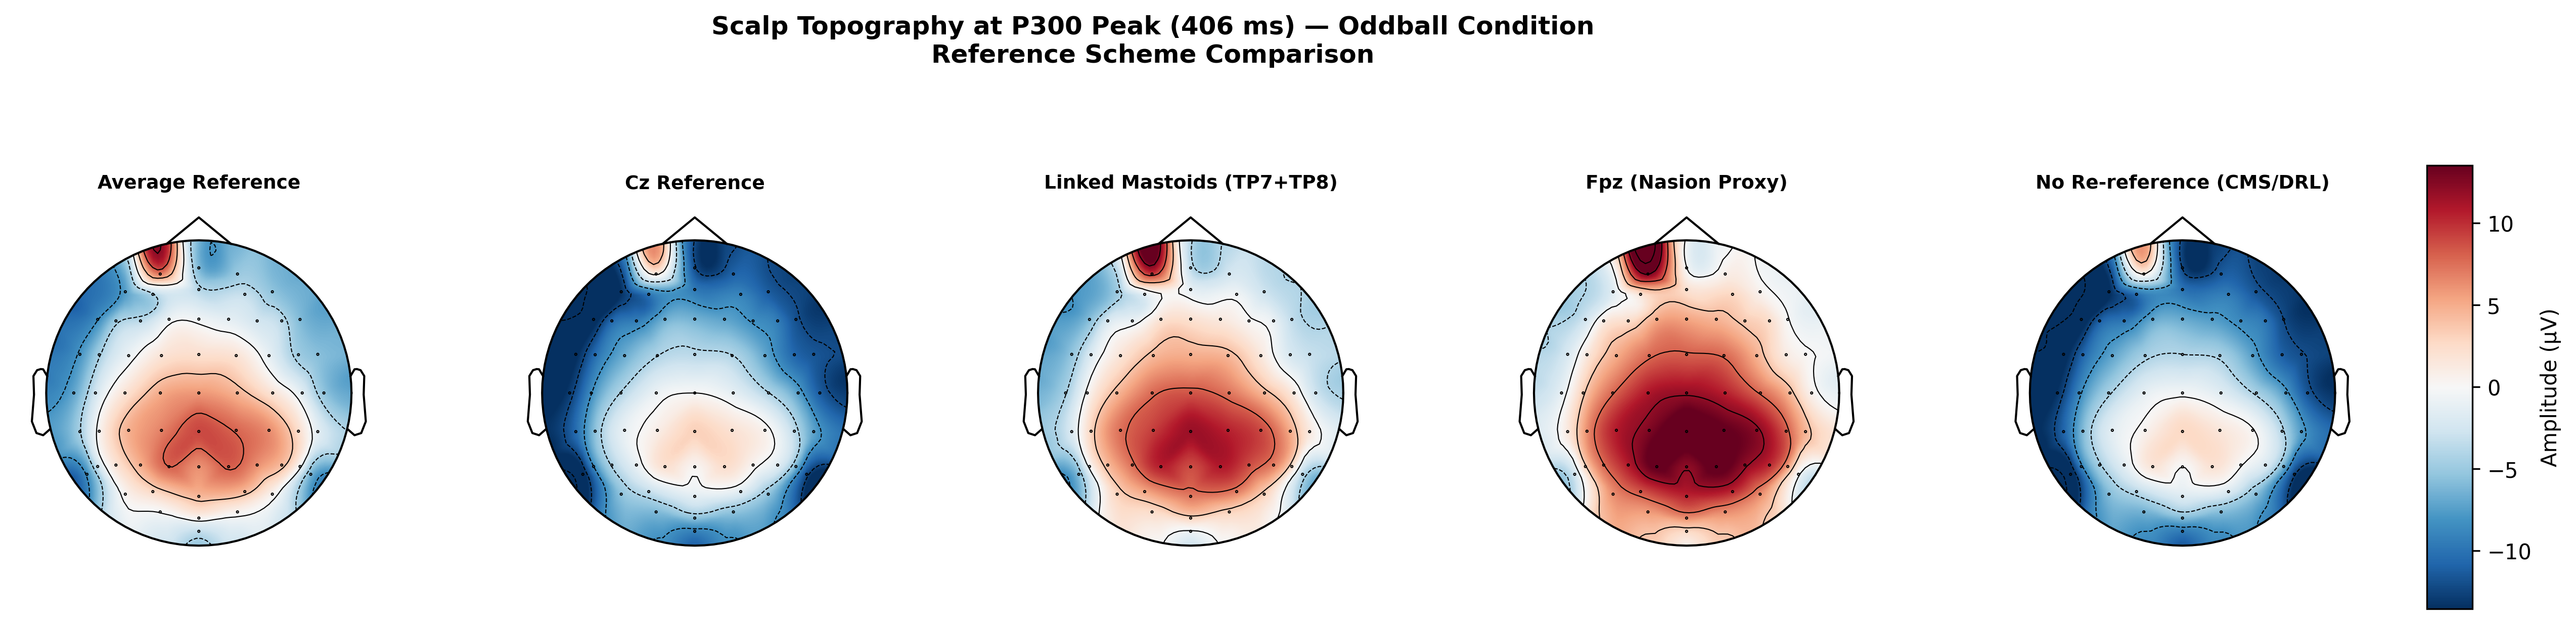
\includegraphics[width=0.88\textwidth]{part3_topo_reference_comparison}
    \caption{Scalp topographic maps at 406.2~ms for the oddball condition under five reference
    schemes. All maps share the same colour scale. The centro-parietal P300 positivity is
    most clearly expressed under average reference and linked mastoids.}
    \label{fig:topo_reference}
\end{figure*}

\begin{figure*}[htbp]
    \centering
    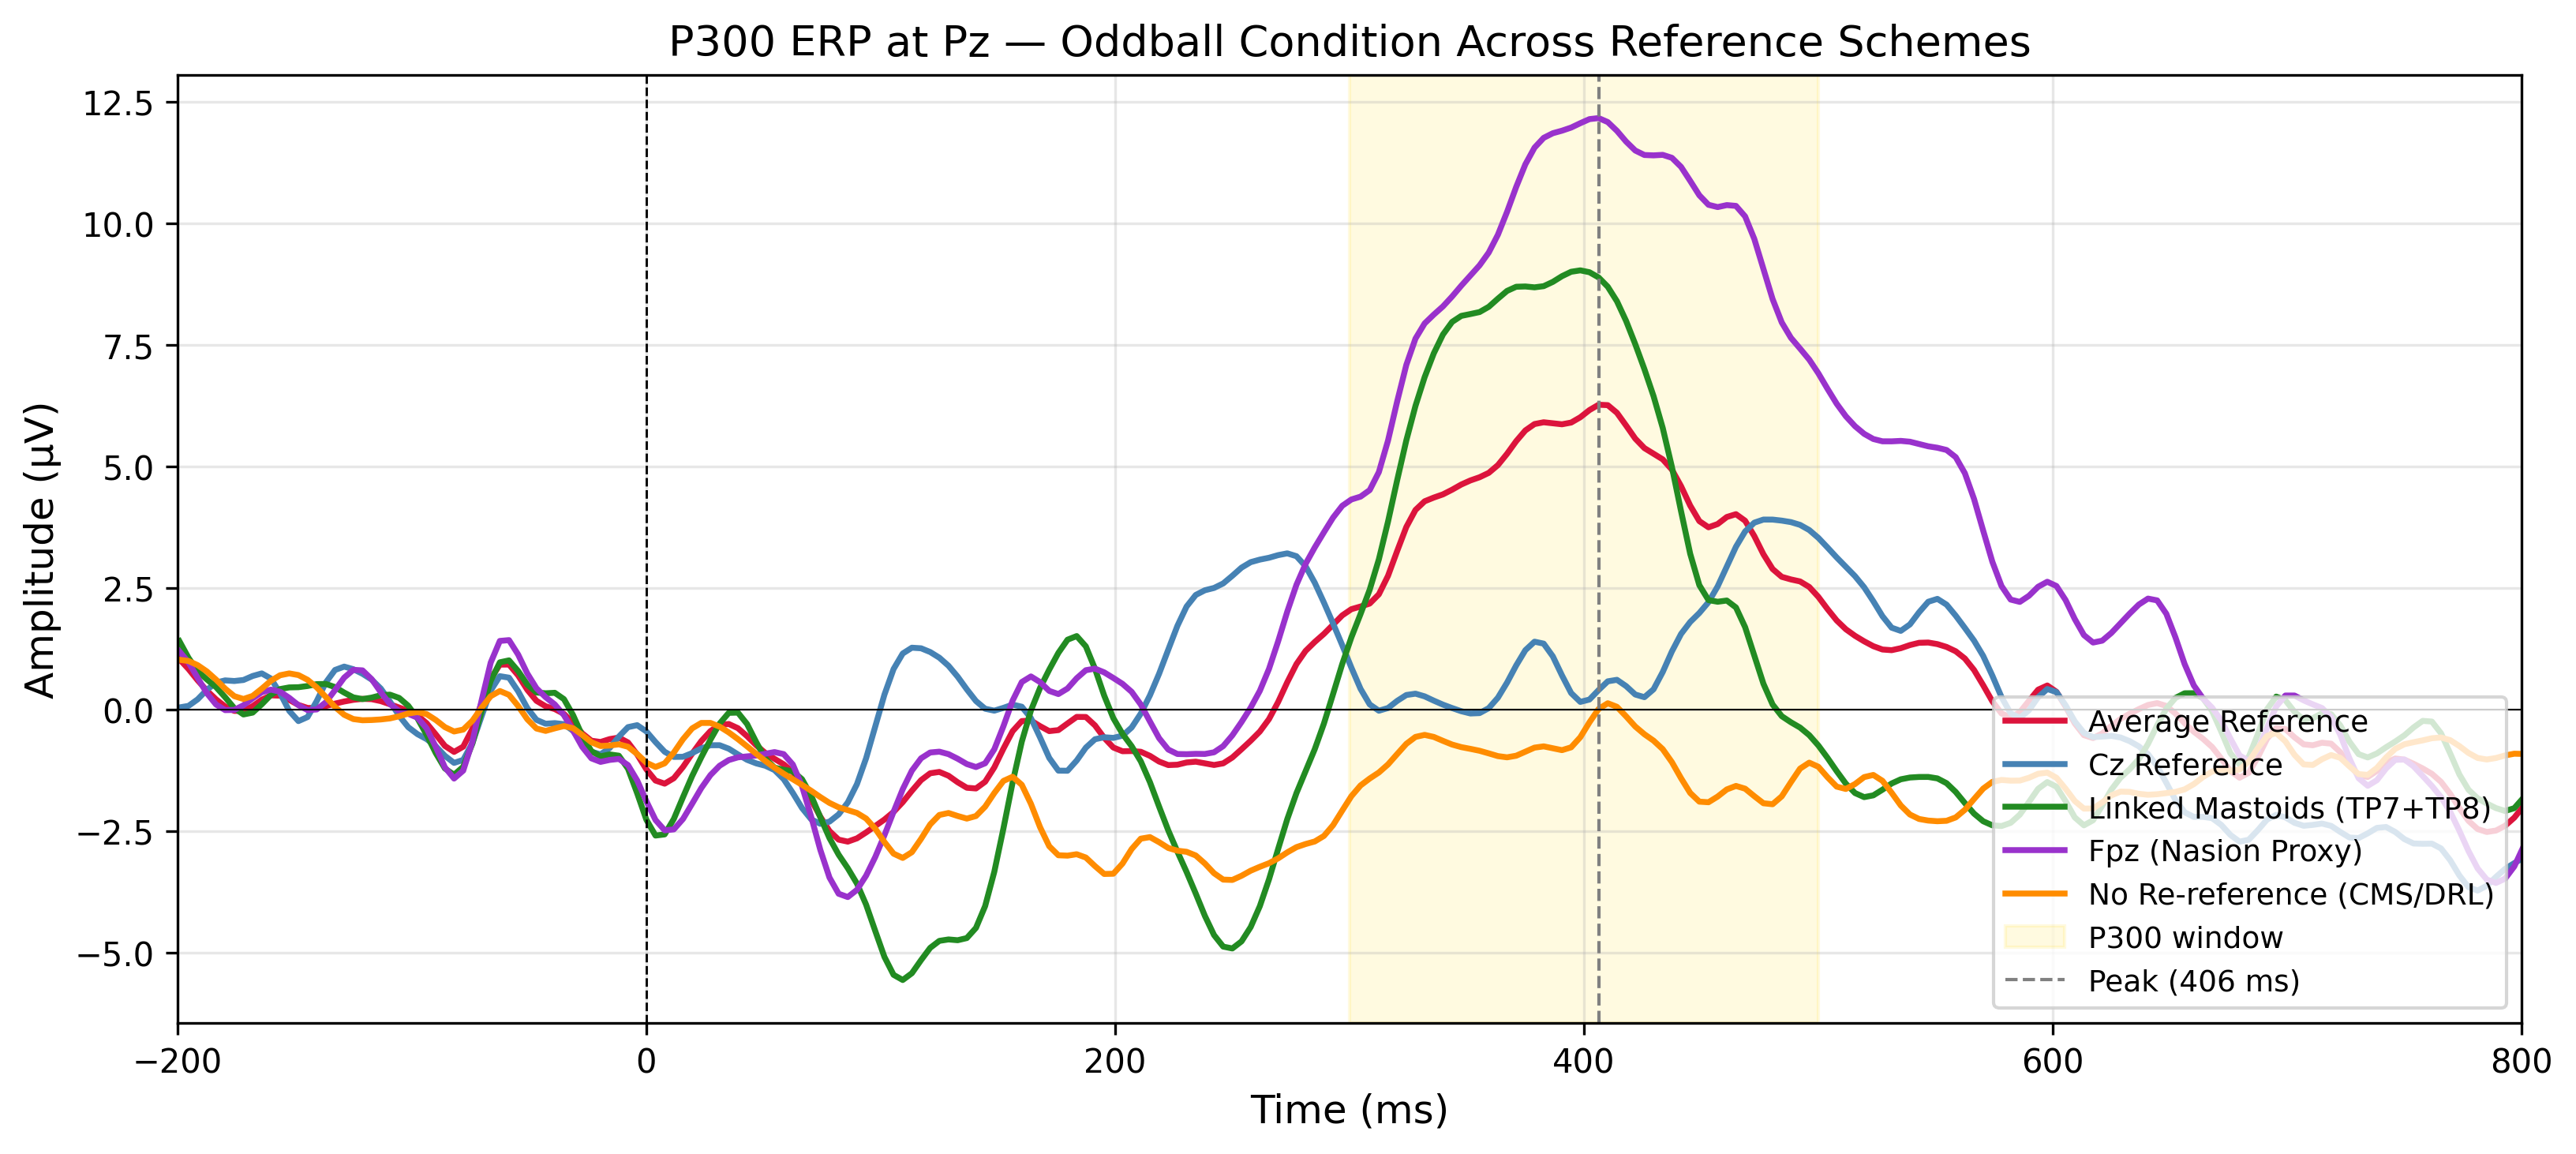
\includegraphics[width=0.82\textwidth]{part3_erp_Pz_reference_comparison}
    \caption{ERP waveforms at Pz under all five reference schemes. Shaded region: P300 window
    (300--500~ms). The CMS/DRL trace is polarity-inverted; the Cz trace is suppressed and latency-shifted.}
    \label{fig:erp_reference}
\end{figure*}

\subsection{Discussion}

\subsubsection{Why Reference Choice Shifts the Apparent Center of Activity}

EEG voltage is always a difference measure. The signal at any electrode
represents the potential difference between that electrode and whatever
site is being used as a reference. When a reference electrode itself
carries neural or artifact signal, that signal is subtracted from every
channel simultaneously, rigidly shifting the entire topographic landscape.
Electrodes close to an active reference appear suppressed, while distant
electrodes may appear paradoxically enhanced. This is not a reflection of
the true neural generator distribution but an artifact of the recording
choice.

\subsubsection{Interpretation of Each Scheme}

\textbf{Average reference} (+4.384~$\mu$V, 406.2~ms): With 64 electrodes
providing dense coverage, the average is a good approximation of the
theoretical infinity reference \citep{Yao2001}. The P300 amplitude
estimate is moderate and the topography shows the expected centro-parietal
maximum with complementary frontal negativity. This is the recommended
standard for topographic ERP analysis with high-density systems
\citep{Luck2005, NunezSrinivasan2006, Hagemann2001}.

\textbf{Cz reference} (+1.280~$\mu$V, 476.6~ms): Cz sits at the vertex,
directly within the P300 topographic maximum. Referencing to Cz subtracts
the P300 signal itself from all channels, reducing the apparent P300
amplitude by 71\% (from 4.384 to 1.280~$\mu$V) and shifting the apparent
peak latency by about 70~ms. The topography under Cz reference shows an
artificially suppressed centro-parietal region, making the P300 appear
weak and peripherally distributed. Cz is a poor choice for any analysis
that targets centro-parietal components.

\textbf{Linked mastoids (TP7+TP8)} (+5.279~$\mu$V, 398.4~ms): The mastoid
electrodes are relatively inactive during the P300 window, making this
a reasonable reference for auditory ERP studies. The amplitude is slightly
inflated compared to average reference because the mastoids carry mild
negativity at this latency, adding a small positive offset to all channels.
The peak latency estimate (398.4~ms) is consistent with average reference.
This reference is acceptable for central and parietal P300 analysis, but
may distort temporal and occipito-temporal topography due to the physical
proximity of TP7/TP8 to those regions \citep{Hagemann2001}.

\textbf{Fpz / nasion reference} (+9.471~$\mu$V, 406.2~ms): This scheme
produces a severely inflated P300 amplitude, more than double the
average-reference estimate. Fpz is susceptible to frontal muscle and
residual blink noise. Using Fpz as a reference injects this frontal
contamination into every channel subtractively, creating an artifactual
large posterior positivity. While the peak latency appears correct
(406.2~ms), the overall amplitude and topographic distribution are
unreliable. The nasion/Fpz reference is generally discouraged for
cognitive ERP research \citep{Nunez1999}.

\textbf{No re-reference} ($-$1.013~$\mu$V, 250.0~ms): Without
re-referencing, the data retains the Biosemi CMS electrode offset, which
is located near POz. This active posterior reference inverts the polarity
of the P300 at Pz (the component appears negative rather than positive)
and the apparent peak at 250~ms likely corresponds to the N2 component
rather than P300. All topographic interpretation from unreferenced Biosemi
data is unreliable and should not be used for publication or analysis
\citep{NunezSrinivasan2006}.

\subsubsection{Best Reference for Occipito-Temporal Sensor Mapping}

The average reference provides the most accurate representation of
occipito-temporal ERP components (P1, N1, N170, P300 temporal contributors
at PO7/PO8). Unlike mastoid referencing, it does not selectively suppress
the lateral temporal and occipito-temporal sensors. Unlike Cz or frontal
references, it does not distort the posterior topography. With 64 channels
and reasonably uniform head coverage, the average reference approximates
the theoretical infinity reference that would be ideal for source
localisation \citep{Yao2001}, and is the consensus recommendation for
high-density EEG topographic analysis \citep{Luck2005, HariPuce2017}.

\section{Conclusion}

This study replicated the canonical P300 ERP in an auditory oddball
paradigm. Preprocessing using automated bad channel rejection (T7),
bandpass filtering (1--40~Hz), 50~Hz notch filtering, and ICA-based
artifact removal produced clean epochs with a 99.2\% retention rate.
The oddball condition produced a robust P3b component peaking at 406.2~ms
at Pz with a mean amplitude of $+4.658\ \mu$V, significantly larger than
both the noise ($d = 1.14$) and standard ($d = 1.46$) conditions,
$F(2, 738) = 103.86$, $p < .001$. The reference comparison demonstrated
that average referencing provides the most accurate and interpretable
topographic representation of the P300 field, whereas Cz referencing
suppresses the component, Fpz referencing inflates it, mastoid referencing
introduces mild distortion, and no re-referencing inverts the polarity
entirely. These findings confirm both the robustness of the P300 as a
neural marker of target detection and the critical importance of reference
choice in ERP topographic analysis.

\bibliographystyle{apalike}
\bibliography{references}

\end{document}
